\thispagestyle{lichsutoanhocnone}
\pagestyle{lichsutoanhoc}
\graphicspath{{../lichsutoanhoc/pic3/}}
\everymath{\color{lichsutoanhoc}}
\blfootnote{$^1$\color{lichsutoanhoc}Viện Toán học, đã nghỉ hưu.}
\blfootnote{$^2$\color{lichsutoanhoc}Hà Nội.}
\begingroup
\AddToShipoutPicture*{\put(0,616){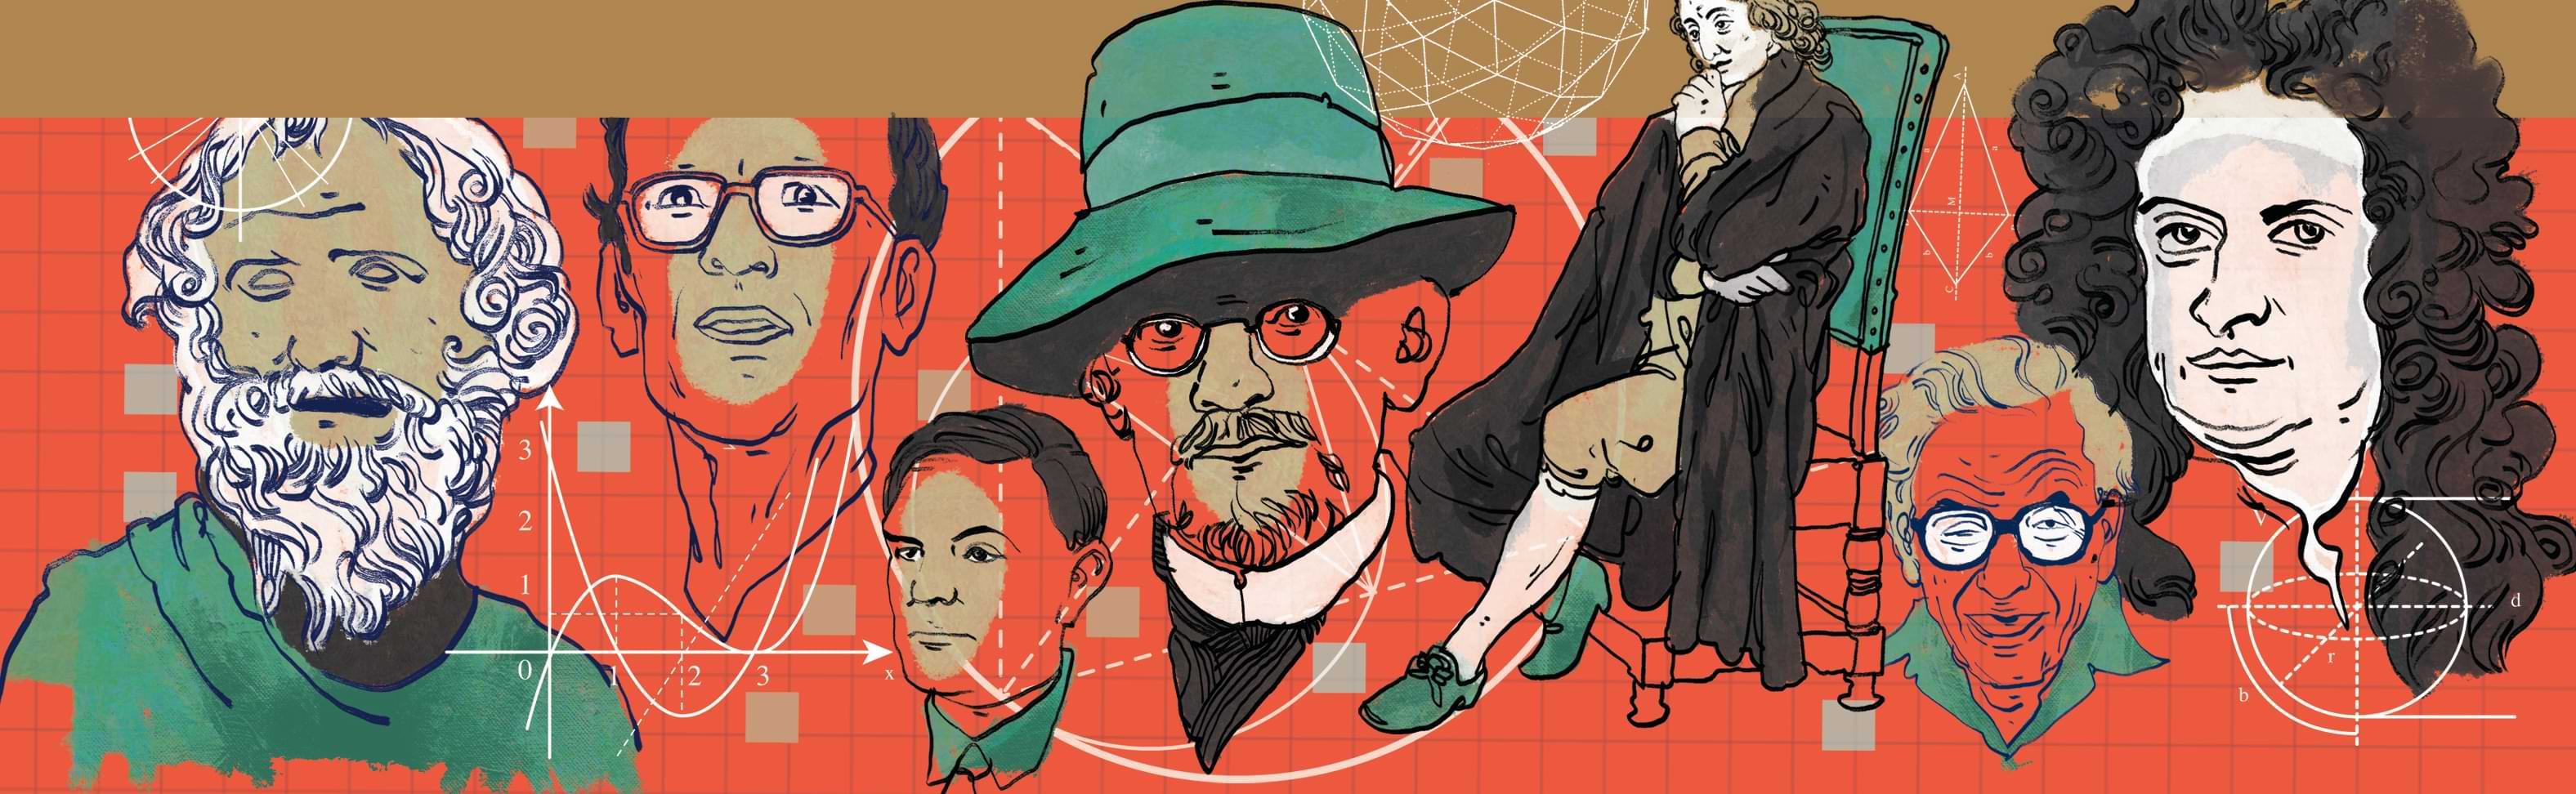
\includegraphics[width=19.3cm]{../bannerlichsu}}}
\AddToShipoutPicture*{\put(56,525){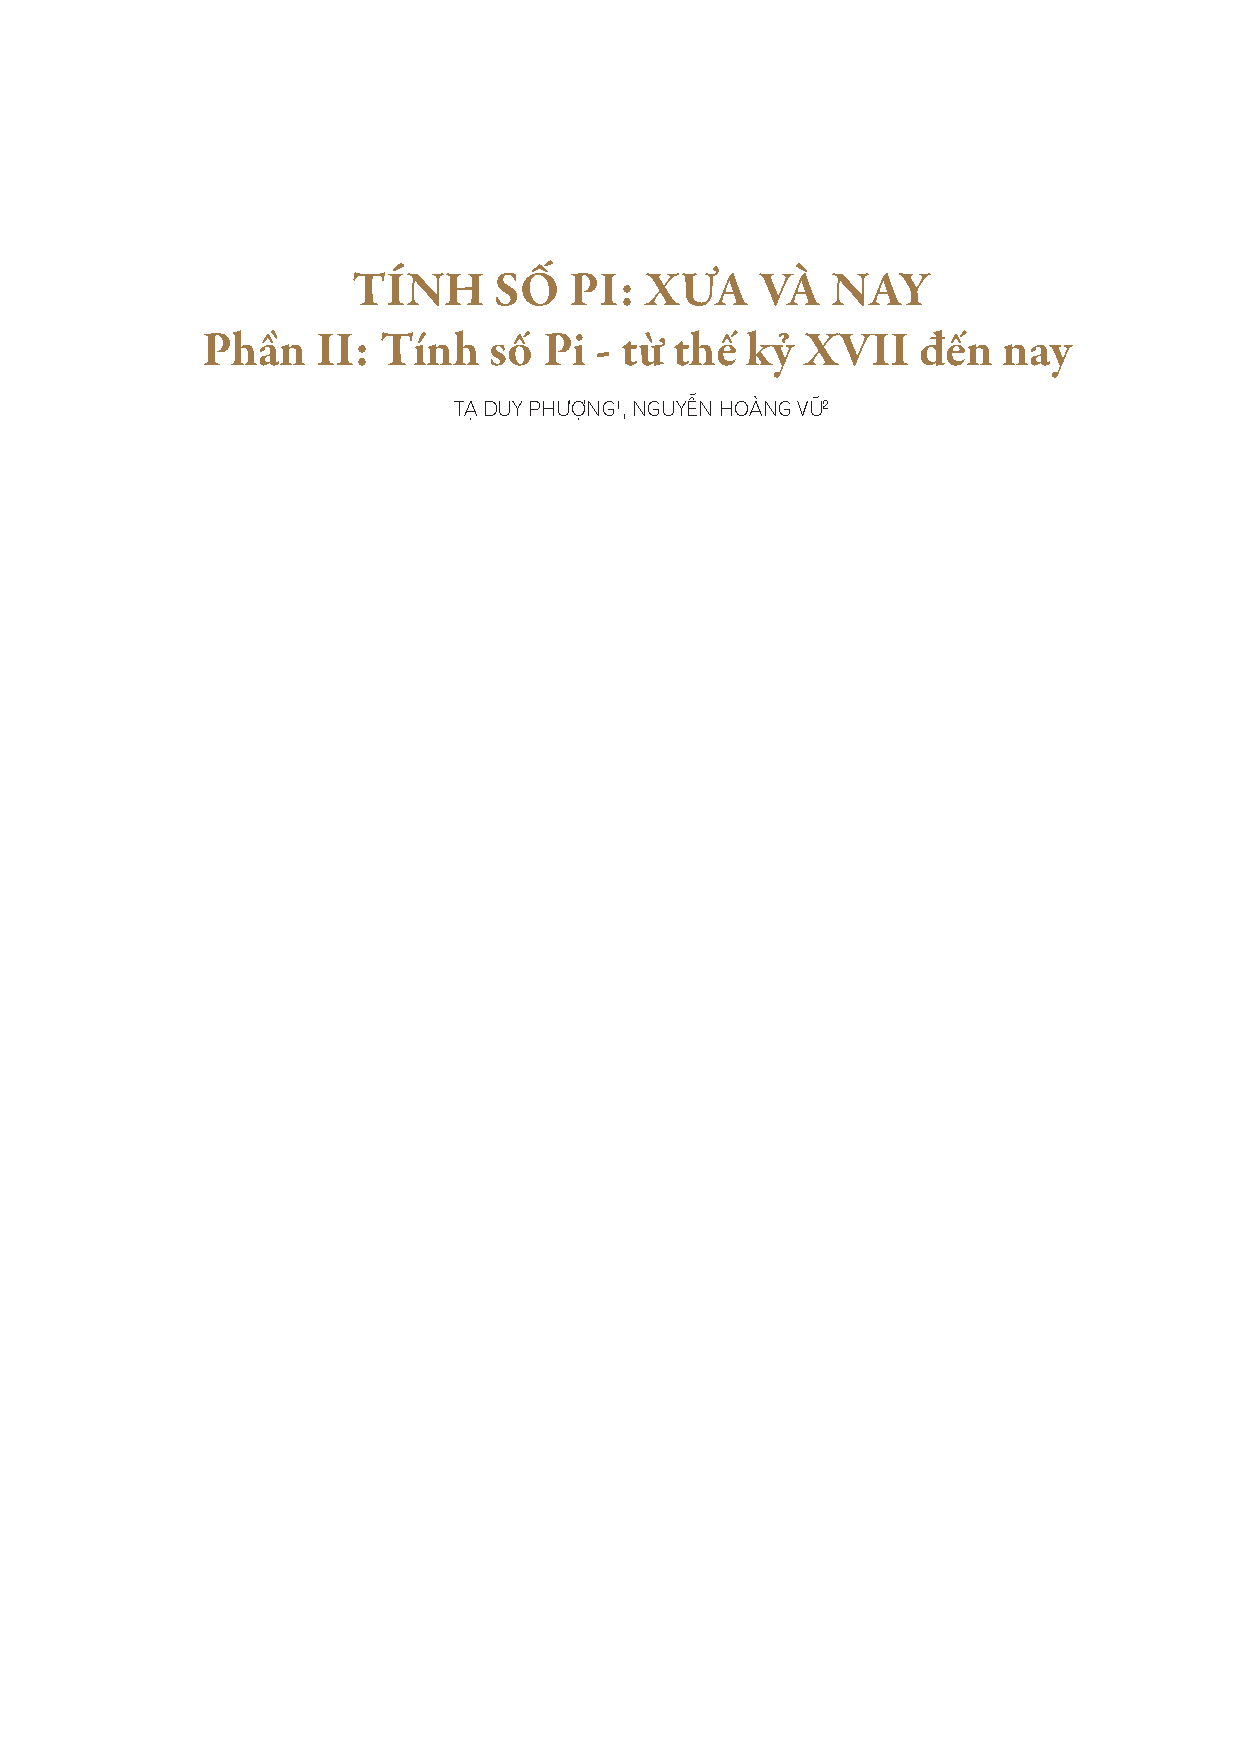
\includegraphics[scale=1]{../tieude.pdf}}}
\centering
\endgroup

\vspace*{185pt}

\begin{multicols}{2}
	\textbf{\color{lichsutoanhoc}Lời dẫn}
	\vskip 0.1cm
	Số $\pi$ chắc chắn là hằng số nổi tiếng và hấp dẫn nhất trong Toán học. 
	\vskip 0.1cm
	Cái tên ``Pi Day--Ngày $\pi$" lần đầu tiên được đề nghị bởi nhà Vật lý Larry Shaw, vào ngày $14$ tháng Ba năm $1988$ ở Bảo tàng Exploratorium, trung tâm San Francisco, vì $3.14$ là giá trị gần đúng của số $\pi$, nó cũng trùng với ngày sinh của Albert Einstein ($14-3-1879$). Kể từ đó, rất nhiều người yêu toán trên thế giới cứ đến $14$ tháng $3$ lại tập trung kỷ niệm hằng số này và qua đó thể hiện tình yêu với toán học. 
	\vskip 0.1cm
	Phần $1$ (Tạp chí Pi, tập $7$, tháng $3-2023$) đã giới thiệu Lịch sử tính số Pi cho tới thế kỉ XVII với phương pháp tính chủ yếu nhờ thuật toán nhân đôi số cạnh của đa giác đều nội ngoại tiếp hình tròn của Archimedes. Phần $2$ tiếp tục giới thiệu cách tính gần đúng số Pi nhờ các công thức khai triển số $\pi$ dưới dạng chuỗi và trên máy tính, chủ yếu từ thế kỉ XVII cho tới nay.
	\vskip 0.1cm
	\textbf{\color{lichsutoanhoc}Tính gần đúng số Pi dưới dạng chuỗi}
	\vskip 0.1cm
	Madhava $(1340-1425)$, nhà toán học Ấn Độ là người đầu tiên sử dụng công thức chuỗi vô hạn dưới đây để tính số $\pi$: 
	\begin{align*}
		\pi  = \sqrt {12} \sum\limits_{k = 1}^\infty  {\frac{{{{\left( { - 1} \right)}^{k + 1}}}}{{\left( {2k - 1} \right) \cdot {3^{k - 1}}}}}. \tag{$1$}
	\end{align*}
	Công thức ($1$) cũng được Leibniz, nhà toán học Đức tìm ra vào năm $1676$. Công thức ($1$) sau này được gọi là \textit{chuỗi Madhava -- Leibniz}.
	\begin{figure}[H]
		\vspace*{-5pt}
		\centering
		\captionsetup{labelformat= empty, justification=centering}
		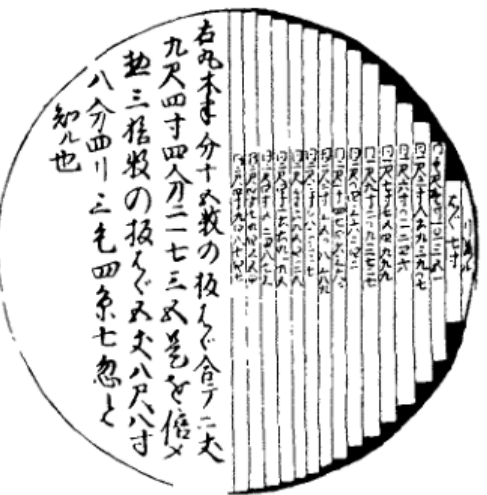
\includegraphics[width= 1\linewidth]{1}
		\caption{\small\textit{\color{lichsutoanhoc}Hình $1$: Kazayuki.}}
		\vspace*{-10pt}
	\end{figure}
	Trong hai cuốn sách của ba nhà toán học Nhật Bản Sawaguchi Kazayuki ($1670$, Hình $1$), Machinag và Ohashi ($1687$, Hình $2$) đã đưa ra công thức ($2$) tính số $\pi$ 
	\begin{align*}
		\pi  = \mathop {\lim }\limits_{n \to \infty } \frac{4}{{{n^2}}}\sum\limits_{j = 1}^n {\sqrt {{n^2} - {j^2}} }. \tag{$2$}
	\end{align*}
	 \begin{figure}[H]
	 	\vspace*{-5pt}
	 	\centering
	 	\captionsetup{labelformat= empty, justification=centering}
	 	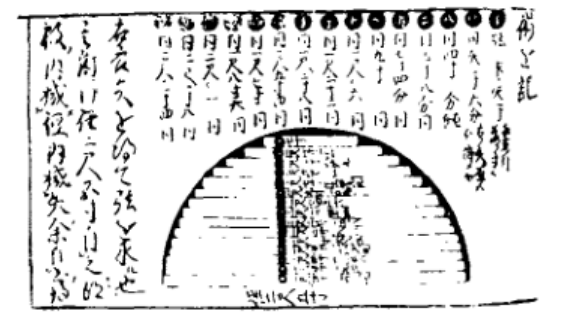
\includegraphics[width= 1\linewidth]{2}
	 	\caption{\small\textit{\color{lichsutoanhoc}Hình $2$: Machinag và Ohashi ($1687$).}}
	 	\vspace*{-10pt}
	 \end{figure}
	\textit{Giải thích công thức} ($2$): Chia $\frac{1}{4}$ hình tròn bán kính $OA= OB = 1$  thành $n$  phần bằng nhau. Vì (Hình $3$) mỗi dải chữ nhật có chiều rộng bằng $\frac{1}{n}$  và chiều dài bằng (theo Định lý Pythagoras) $\sqrt{1- \left(\frac{j}{n}\right)^2}$ nên diện tích của dải chữ nhật thứ  $j$ bằng	 
	\begin{align*}
		{S_j} = \frac{1}{n}\sqrt {1 - {{\left( {\frac{j}{n}} \right)}^2}}  = \frac{1}{{{n^2}}}\sqrt {{n^2} - {j^2}}.
	\end{align*}
	\begin{figure}[H]
		\vspace*{-5pt}
		\centering
		\captionsetup{labelformat= empty, justification=centering}
		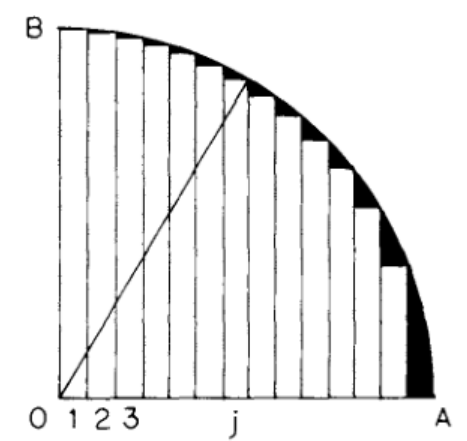
\includegraphics[width= 1\linewidth]{3}
		\caption{\small\textit{\color{lichsutoanhoc}Hình $3$.}}
		\vspace*{-10pt}
	\end{figure}
	Tổng diện tích các hình chữ nhật bằng 
	\begin{align*}
		{S_n} = \sum\limits_{i = 1}^n {{S_i} = } \frac{1}{{{n^2}}}\sum\limits_{j = 1}^n {\sqrt {{n^2} - {j^2}} }.
	\end{align*}
	Khi $n \to \infty$ thì $S_n$ tiến tới diện tích ($= \frac{\pi}{4}$) của $\frac{1}{4}$ hình tròn bán kính $=1$.  Suy ra công thức ($2$).
	\vskip 0.1cm
	Về mặt lý thuyết, theo công thức ($2$), người Nhật có thể tính gần đúng số $\pi$ với độ chính xác bất kỳ khi chọn số $n$ đủ lớn. Tuy nhiên, chuỗi này hội tụ rất chậm vì phải khai căn, giống như trong phương pháp của Archimedes hoặc công thức của François Viète (xem [$1$]).
	\vskip 0.1cm
	Chưa có cơ sở để khẳng định người Nhật đã thực sự sử dụng công thức ($2$) để tính gần đúng số $\pi$. Tuy nhiên, John Wallis đã tiếp cận tương tự: Vì $\frac{1}{4}$ đường tròn tâm $O$ bán kính bằng $1$ trong góc phần tư thứ nhất có phương trình $y = \sqrt{1- x^2}$ có diện tích bằng $\frac{\pi}{4}$ nên theo ngôn ngữ tích phân hiện đại:  
	\begin{align*}
		\frac{\pi }{4} = \int\limits_0^1 {\sqrt {1 - {x^2}} dx} .
	\end{align*}   
	John Wallis trong cuốn \textit{Arithmetica infinitorum} ($1655$) đã rất vất vả để tìm ra công thức mà bây giờ được gọi là \textit{tích Wallis} hay \textit{tích vô hạn}:
	\begin{align*}
		\frac{\pi }{2} = \frac{2}{1} \cdot \frac{2}{3} \cdot \frac{4}{3} \cdot \frac{4}{5} \cdot \frac{6}{5} \cdot \frac{6}{7} \cdot \frac{8}{7} \cdot \frac{8}{9}... \tag{$3$}
	\end{align*}
	Ngày nay, nhờ kỹ thuật tính tích phân từng phần, học sinh lớp $12$ cũng có thể chứng minh được 
	\begin{align*}
		\int\limits_0^{\frac{\pi }{2}} {{{\sin }^{2m}}xdx = \frac{{1 \cdot 3 \cdot 5 \cdot ... \cdot \left( {2m - 1} \right)}}{{2 \cdot 4 \cdot 6 \cdot ...2m}}} \frac{\pi }{2}
	\end{align*}
	và
	\begin{align*}
		\int\limits_0^{\frac{\pi }{2}} {{{\sin }^{2m + 1}}xdx = \frac{{2 \cdot 4 \cdot 6 \cdot ... \cdot 2m}}{{1 \cdot 3 \cdot 5 \cdot ...\left( {2m + 1} \right)}}} .
	\end{align*}
	Lấy giới hạn hai vế khi $m \to \infty$, và vì vế trái của chúng bằng nhau, nên vế phải  bằng nhau và ta suy ra công thức Wallis ($3$).
	\vskip 0.1cm
	Công thức Wallis là một cột mốc quan trọng trong lịch sử tính số $\pi$: Wallis là người đầu tiên trong lịch sử tìm ra chuỗi vô hạn chỉ gồm các phép tính đơn giản, không có căn bậc hai gây khó khăn khi tính toán bằng số như trong các công thức của Archimedes hoặc Viète.  
	\vskip 0.1cm
	Vào những năm $1660$, nhà khoa học người Anh Isaac Newton  và nhà toán học người Đức Gottfried Wilhelm Leibniz đã xây dựng phép toán vi phân (calculus), dẫn tới phát hiện rât nhiều chuỗi vô hạn cho phép tính số $\pi$.
	\vskip 0.1cm  
	Vào năm $1672$, James Gregory và Gottfried Leibnitz năm $1674$, độc lập nhau, đã đưa ra công thức (ngày nay được gọi là công thức Gregory -- Leibnitz) tính arctan của  $t, 0 \le t\le 1$:
	\begin{align*}
		\arctan t = t - \frac{{{t^3}}}{3} + \frac{{{t^5}}}{5} - \frac{{{t^7}}}{7} + \frac{{{t^9}}}{9} - ... \tag{$4$}
	\end{align*}
	\textit{Giải thích:} Ta có 
	\begin{align*}
		\arctan t = \int\limits_0^t {\frac{1}{{1 + {x^2}}}dx} .
	\end{align*}
	Vì $\frac{1}{{1 + u}} = 1 - u + {u^2} - {u^3} + ...$   nên
	\begin{align*}
			\int\limits_0^t {\frac{1}{{1 + {x^2}}}dx}  &= \int\limits_0^t {\left( {1 - {x^2} + {x^4} - {x^6} + ...} \right)dx} \\
			&= t - \frac{{{t^3}}}{3} + \frac{{{t^5}}}{5} - \frac{{{t^7}}}{7} + ...
	\end{align*}
	Suy ra công thức Gregory -- Leibnitz ($4$).
	\vskip 0.1cm 
	Cho $t = 1$  ta có
	\begin{align*}
		\frac{\pi }{4} = \arctan 1 = 1 - \frac{1}{3} + \frac{1}{5} - \frac{1}{7} + \frac{1}{9} + ...
	\end{align*}
	Tuy nhiên, chuỗi này hội tụ rất chậm, thí dụ, cần phải tính hơn $300$ số hạng để nhận được số $\pi$ chính xác đến hai chữ số thập phân, và số gần đúng này không chính xác bằng $3\frac{1}{7}$,  giá trị mà Archimedes đã nhận được hơn $2000$ năm trước.
	\vskip 0.1cm
	Vì vậy, cần xem xét công thức ($4$) tỷ mỉ hơn.
	\vskip 0.1cm
	Năm $1699$, nhà toán học người Anh Abraham Sharp đã dùng chuỗi Gregory -- Leibnitz ($4$) với $t = \frac{1}{\sqrt{3}}$ để tính số $\pi$ chính xác đến $71$ chữ số:
	\begin{align*}
		\frac{\pi }{6} &= \arctan \frac{1}{{\sqrt 3 }} \\
		&= \frac{1}{{\sqrt 3 }}\left( {1 - \frac{1}{{3 \cdot 3}} + \frac{1}{{5 \cdot {3^2}}} - ...} \right) \tag{$5$}
	\end{align*}
	Kỷ lục này phá vỡ kỉ lục tính gần đúng số $\pi$ đến $39$ chữ số được thiết lập nhờ thuật toán Archimedes và cho thấy sức mạnh của Giải tích.   
	\vskip 0.1cm
	Năm $1719$, nhà toán học người Pháp de Lagny đã tính gần đúng số $\pi$ đến $127$ chữ số thập phân (có $100$ chữ số chính xác) nhờ chuỗi Sharp ($5$).
	\vskip 0.1cm 
	Năm $1706$, John Machin ($1680-1752$) sử dụng mẹo sau đây để tăng tốc độ hội tụ của chuỗi Gregory -- Leibnitz ($4$): Với $\tan \beta = \frac{1}{5}$ ta có 
	\begin{align*}
		\tan 2\beta  = \frac{{2\tan \beta }}{{1 - {{\tan }^2}\beta }} = \frac{5}{{12}}
	\end{align*}
	và 
	\begin{align*}
		\tan 4\beta  = \frac{{2\tan 2\beta }}{{1 - {{\tan }^2}2\beta }} = \frac{{120}}{{119}}.
	\end{align*}
	Suy ra 
	\begin{align*}
		\tan \left( {4\beta  - \frac{\pi }{4}} \right) &= \frac{{\tan 4\beta  - \tan \frac{\pi }{4}}}{{1 + \tan 4\beta \tan \frac{\pi }{4}}} = \frac{{\frac{{120}}{{119}} - 1}}{{1 + \frac{{120}}{{119}}}} \\
		&= \frac{1}{{239}}.
	\end{align*}
	Vậy 
	\begin{align*}
		\arctan \frac{1}{{239}} = 4\beta  - \frac{\pi }{4} = 4\arctan \frac{1}{5} - \frac{\pi }{4}.
	\end{align*}
	Áp dụng công thức ($4$) ta được
	\begin{align*}
			\!\!\!\!\!\!\frac{\pi }{4} = &4\arctan \frac{1}{5} - \arctan \frac{1}{{239}} \\
			= &4\left( {\frac{1}{5} - \frac{1}{{3 \cdot {5^3}}} + \frac{1}{{5 \cdot {5^5}}} - ...} \right) \\
			&-\!\! \left(\!\! {\frac{1}{{239}} \!-\! \frac{1}{{3 \!\cdot\! {{239}^3}}} \!+\! \frac{1}{{5 \!\cdot\! {{239}^5}}} \!-\! ....}\!\! \right)\!\!. \tag{$6$}
	\end{align*}
	Vì $239$ là đủ lớn, nên $\arctan\frac{1}{239}$ là số đủ nhỏ. Hơn nữa, do các số hạng liên tiếp trong phân tích chuỗi $\arctan\frac{1}{5}$ chỉ chênh nhau một đại lượng $\frac{1}{5^2} = 0.04$ nên có thể dễ dàng tính bằng tay $\arctan \frac{1}{5}$. Từ nhận xét này, John Machin đã tính bằng tay xấp xỉ số $\pi$ đến $100$ chữ số. 
	\vskip 0.1cm
	Dưới đây là một số công thức được Euler ($1707-1783$) phát hiện và trình bày trong cuốn sách \textit{Introductio in Analysin infinitorum} ($1748$).
	\vskip 0.1cm
	Từ công thức đã được Newton chúng minh
	\begin{align*}
		\sin x = x - \frac{{{x^3}}}{{3!}} + \frac{{{x^5}}}{{5!}} - \frac{{{x^7}}}{{7!}} + ...,
	\end{align*}
	Euler đặt $x^2 = y$ và xét phương trình 
	\begin{align*}
		\sin x = 0 \tag{$7$}
	\end{align*}
	như phương trình bậc vô hạn, ta có (với $y \ne 0 $):
	\begin{align*}
		1 - \frac{y}{{3!}} + \frac{{{y^2}}}{{5!}} - \frac{{{y^3}}}{{7!}} + .... = 0. \tag{$8$}
	\end{align*}
	Nghiệm của phương trình ($7$) là $0, \pm \pi, \pm 2\pi, \ldots$  Do đó nghiệm của ($8$) là $\pi^2, (2\pi)^2, \ldots$
	\vskip 0.1cm  
	Theo tính chất của phương trình bậc vô hạn, tổng nghịch đảo của các nghiệm của ($8$) bằng ngược dấu hệ số của $y$, tức là
	\begin{align*}
		\frac{1}{{{\pi ^2}}} + \frac{1}{{{{\left( {2\pi } \right)}^2}}} + \frac{1}{{{{\left( {3\pi } \right)}^2}}} + .... = \frac{1}{{3!}}
	\end{align*}
	hay 
	\begin{align*}
		1 + \frac{1}{{{2^2}}} + \frac{1}{{{3^2}}} + .... = \frac{{{\pi ^2}}}{6}. \tag{$9$}
	\end{align*}
	Lưu ý rằng Jacques Bernoulli (và cả Leibniz) tuy chứng minh được sự hội tụ của chuỗi ($9$), nhưng đã không tính được tổng này. 
	\vskip 0.1cm
	Tương tự cho $\cos x$,  Euler tính được
	\begin{align*}
		\frac{{{\pi ^2}}}{8} = \frac{1}{{{1^2}}} + \frac{1}{{{3^2}}} + \frac{1}{{{5^2}}} + .... \tag{$10$}
	\end{align*}
	Nhân ($10$) với $2$ và trừ cho ($9$), ta đươc
	\begin{align*}
		\frac{{{\pi ^2}}}{{12}} = \frac{1}{{{1^2}}} - \frac{1}{{{2^2}}} + \frac{1}{{{3^2}}} - \frac{1}{{{4^2}}} + \frac{1}{{{5^2}}} + ....
	\end{align*}
	Euler đã dùng công thức
	\begin{align*}
		\frac{\pi^2}{6} = \frac{2^2}{2^2 - 1} \cdot \frac{3^2}{3^2 - 1} \cdot \frac{5^2}{5^2 - 1} \cdot \frac{7^2}{7^2 - 1} \cdot ...
	\end{align*}
	để tính logarithm của $\pi$.
	\vskip 0.1cm  
	Euler cũng đã chứng minh công thức
	\begin{align*}
		{\rm{arctan}}\frac{1}{p}\! =\! \arctan \frac{1}{{p \!+\! q}} \!+\! \arctan \frac{q}{{{p^2} \!+\! pq \!+\! 1}}.
	\end{align*}
	Cho $p = q = 1$ ta được 
	\begin{align*}
		\frac{\pi }{4} = \arctan 1 = \arctan \frac{1}{2} + \arctan \frac{1}{3}.
	\end{align*}
	Tính $\arctan \frac{1}{7}$  và  $\arctan \frac{3}{{79}}$ trong công thức
	\begin{align*}
		\pi  = 20\arctan \frac{1}{7} + 8\arctan \frac{3}{{79}}
	\end{align*}
	theo công thức hội tụ nhanh
	\begin{align*}
		\arctan x \!=\! \frac{y}{x}\left( {1 \!+\! \frac{2}{3}y \!+\! \frac{{2 \!\cdot\! 4}}{{3 \!\cdot\! 5}}{y^2} \!+\! \frac{{2 \!\cdot \!4 \!\cdot\! 6}}{{3 \!\cdot\! 5 \!\cdot\! 7}}{y^3} \!+\! ...} \right)
	\end{align*}
	với $y = \frac{{{x^2}}}{{1 + {x^2}}},$  Euler đã tính gần đúng số $\pi$  đến $20$ chữ số trong vòng $1$ giờ.
	\vskip 0.1cm
	Trên đây chỉ là một số trong rất nhiều công thức của Euler tính gần đúng số $\pi$  theo chuỗi.
	\vskip 0.1cm
	\textbf{\color{lichsutoanhoc}Phụ lục $\pmb1$. Một số công thức tính số} $\pmb{\pi}$ ([$3$])
	\vskip 0.1cm
	$\pmb1$\textbf{\color{lichsutoanhoc}. Archimedes} (khoảng $250$ trước công nguyên)
	\vskip 0.1cm
	Đặt  $P_6 := 4\sqrt{3}, p_6 = 6$ là chu vi lục giác đều ngoại tiếp và nội tiếp đường tròn bán kính $1$ và
	\begin{align*}
		{P_{2n}}: = \frac{{{P_n}{p_n}}}{{{P_n} + {p_n}}}, {p_{2n}}: = \sqrt {{P_{2n}}{p_n}} 
	\end{align*}
	là chu vi đa giác đều ngoại tiếp và nội tiếp đường tròn bán kính $1$ khi gấp đôi số cạnh. Khi ấy (xem [$1$])  $\mathop {\lim }\limits_{n \to \infty } {P_n} = \mathop {\lim }\limits_{n \to \infty } {p_n} = \pi$.
	\vskip 0.1cm
	Nhờ công thức này, Archimedes đã chứng minh được $3\frac{10}{71} < \pi < 3\frac{10}{70}$ và nhà toán học người Áo Christoph Grienberger năm $1630$ đã đạt kỷ lục tính chính xác  số $\pi$  đến $39$ chữ số (xem [$1$]).
	\vskip 0.1cm
	$\pmb2$\textbf{\color{lichsutoanhoc}. Francois Viète} (khoảng $1578$)
	\begin{align*}
		\frac{2}{\pi } =& \sqrt {\frac{1}{2}}  \cdot \sqrt {\frac{1}{2}\left( {1 + \sqrt {\frac{1}{2}} } \right)}  \\
		&\cdot \sqrt {\frac{1}{2}\left( {1 + \sqrt {\frac{1}{2}\left( {1 + \sqrt {\frac{1}{2}} } \right)} } \right)} ...,
	\end{align*}
	Nhờ công thức này, nhà toán học François Viète năm $1578$ đã tính chính xác số $\pi$  đến $9$ chữ số.
	\vskip 0.1cm
	$\pmb3$\textbf{\color{lichsutoanhoc}. John Wallis} (khoảng $1655$)
	\begin{align*}
		\frac{\pi }{2} = \frac{2}{1} \cdot \frac{2}{3} \cdot \frac{4}{3} \cdot \frac{4}{5} \cdot \frac{6}{5} \cdot \frac{6}{7} \cdot \frac{8}{7} \cdot \frac{8}{9}...
	\end{align*}
	$\pmb4$\textbf{\color{lichsutoanhoc}. William Brouncker} (khoảng $1658$)
	\begin{align*}
		\pi  = \frac{4}{{1 + \frac{1}{{2 + \frac{9}{{2 + \frac{{25}}{{2 + ...}}}}}}}}
	\end{align*}
	$\pmb5$\textbf{\color{lichsutoanhoc}. Mādhava, Gregory, Leibnitz} ($1450-1671$)
	\begin{align*}
		\frac{\pi }{2} = 1 - \frac{1}{3} + \frac{1}{5} - \frac{1}{7} + ...
	\end{align*}
	$\pmb6$\textbf{\color{lichsutoanhoc}. Isaac Newton} (khoảng $1666$)
	\begin{align*}
		\pi  =& \frac{{3\sqrt 3 }}{4} \\
		&+\! 24\left(\!\! {\frac{1}{{12}} \!-\! \frac{1}{{5 \!\cdot\! {2^5}}} \!-\! \frac{1}{{28 \!\cdot\! {2^7}}} \!-\! \frac{1}{{72 \!\cdot\! {2^9}}} \!-\! ...}\! \right)
	\end{align*}
	Năm $1665$, Isaac Newton đã tính chính xác số $\pi$ đến $16$ chữ số thập phân.
	\vskip 0.1cm
	$\pmb7$\textbf{\color{lichsutoanhoc}. Công thức kiểu Machin} ($1706-1776$)
	\begin{align*}
		&\frac{\pi }{4} = 4\arctan \left( {\frac{1}{5}} \right) - \arctan \left( {\frac{1}{{239}}} \right);\\
		&\frac{\pi }{4} = \arctan \left( {\frac{1}{2}} \right) + \arctan \left( {\frac{1}{3}} \right);\\
		&\frac{\pi }{4} = 2\arctan \left( {\frac{1}{2}} \right) - \arctan \left( {\frac{1}{7}} \right);\\
		&\frac{\pi }{4} = 2\arctan \left( {\frac{1}{3}} \right) + \arctan \left( {\frac{1}{7}} \right).
	\end{align*}
	Năm $1706$, Machin đã tính chính xác số $\pi$  đến $100$ chữ số thập phân.
	\vskip 0.1cm
	$\pmb8$\textbf{\color{lichsutoanhoc}. Leonard Euler} (khoảng $1748$)
	\begin{align*}
		\frac{{{\pi ^2}}}{6} &= 1 + \frac{1}{{{2^2}}} + \frac{1}{{{3^2}}} + \frac{1}{{{4^2}}} + \frac{1}{{{5^2}}} + ...;\\
		\frac{{{\pi ^4}}}{{90}} &= 1 + \frac{1}{{{2^4}}} + \frac{1}{{{3^4}}} + \frac{1}{{{4^4}}} + \frac{1}{{{5^4}}} + ...;\\
		\frac{{{\pi ^2}}}{6} &= 3\sum\limits_{m = 1}^\infty  {\frac{1}{{{m^2}\left( \begin{array}{l}
						2m\\
						m
					\end{array} \right)}}} .
	\end{align*}
	$\pmb9$\textbf{\color{lichsutoanhoc}. Srinivasa Ramanujan} ($1914$)
	\begin{align*}
		&\frac{1}{\pi } = {\sum\limits_{n = 0}^\infty  {\left( \begin{array}{l}
					2n\\
					n
				\end{array} \right)} ^2}\frac{{42n + 5}}{{{2^{12n + 4}}}};\\
		&\frac{1}{\pi } = \frac{{\sqrt 8 }}{{9801}}\sum\limits_{n = 0}^\infty  {\frac{{\left( {4n} \right)!}}{{{{\left( {n!} \right)}^4}}}} \frac{{\left( {1103 + 26390n} \right)}}{{{{396}^{4n}}}}.
	\end{align*}
	$\pmb10$\textbf{\color{lichsutoanhoc}. Louis Comtet} ($1974$)
	\begin{align*}
		\frac{{{\pi ^4}}}{{90}} = \frac{{36}}{{17}}\sum\limits_{m = 1}^\infty  {\frac{1}{{{m^4}\left( \begin{array}{l}
						2m\\
						m
					\end{array} \right)}}.} 
	\end{align*}
	$\pmb11$\textbf{\color{lichsutoanhoc}. Eugene Salamin, Richard Brent} ($1976$)
	\vskip 0.1cm
	Đặt $a_0 := 1, b_0 = \frac{1}{\sqrt{2}}, s_0 = \frac{1}{2}$.
	\vskip 0.1cm     
	Với $k = 1,2,3, \ldots$ tính 
	\begin{align*}
		&{a_k} = \frac{{{a_{k - 1}} + {b_{k - 1}}}}{2}, {b_k} = \sqrt {{a_{k - 1}}{b_{k - 1}}} ,\\
		& {c_k} = a_k^2 - b_k^2, {s_k} = {s_{k - 1}} - {2^k}{c_k}, \\
		&{p_k} = \frac{{2a_k^2}}{{{s_k}}}.
	\end{align*}
	Khi ấy $\mathop {\lim }\limits_{k \to \infty } {p_k} = \pi$   và tốc độ hội tụ là cấp hai. 
	\vskip 0.1cm
	$\pmb{12.}$ \textbf{\color{lichsutoanhoc}Ronathan Borwein, Peter Borwein} ($1985$)
	\vskip 0.1cm
	Đặt ${a_0} = 6 - 4\sqrt 2 ,\;{y_0} = \sqrt 2  - 1.$  
	\vskip 0.1cm
	Với $k = 1,2,3,\ldots$ tính 
	\begin{align*}
		{y_{k + 1}} =& \frac{{1 - \sqrt[4]{{1 - y_k^4}}}}{{1 + \sqrt[4]{{1 - y_k^4}}}},\\
		{a_{k + 1}} =& {a_k}{\left( {1 + {y_{k + 1}}} \right)^4} \\
		&- {2^{2k + 3}}{y_{k + 1}}\left( {1 + {y_{k + 1}} + y_{k + 1}^2} \right).
	\end{align*}
	Khi ấy $\mathop {\lim }\limits_{k \to \infty } {a_k} = \frac{1}{\pi }$  và tốc độ hội tụ là cấp hai.
	\vskip 0.1cm
	$\pmb{13.}$ \textbf{\color{lichsutoanhoc}Ronathan Borwein, Peter Borwein} ($1985$)
	\vskip 0.1cm
	Hệ thức sau đây không đúng nhưng chính xác đến $42$ tỷ chữ số thập phân
	\begin{align*}
		\pi  = {\left( {\frac{1}{{{{10}^5}}}\sum\limits_{n =  - \infty }^\infty  {{e^{ - \frac{{{n^2}}}{{{{10}^{10}}}}}}} } \right)^2}.
	\end{align*}
	$\pmb{14.}$ \textbf{\color{lichsutoanhoc}David Chudnovsky, Gregory Chudnovsky} ($1989$)
	\begin{align*}
		\frac{1}{\pi } =& 12\sum\limits_{n = 0}^\infty  {{{\left( { - 1} \right)}^n}\frac{{\left( {6n} \right)!}}{{{{\left( {n!} \right)}^3}\left( {3n} \right)!}}} \\
		&\times\frac{{13591409 + n545140134}}{{{{\left( {{{640320}^3}} \right)}^{n + \frac{1}{2}}}}}.
	\end{align*}
	$\pmb{15.}$ \textbf{\color{lichsutoanhoc}Ronathan Borwein, Peter Borwein} ($1989$)
	\begin{align*}
		\frac{1}{\pi } = 12\sum\limits_{n = 0}^\infty  {\frac{{{{\left( { - 1} \right)}^n}\left( {6n} \right)!}}{{{{\left( {n!} \right)}^3}\left( {3n} \right)!}}} \frac{{\left( {A + nB} \right)}}{{{C^{n + \frac{1}{2}}}}}.
	\end{align*}
	Trong đó 
	\begin{align*}
			A\!:\! &\!=\! 212175710912\sqrt {61}  \!+\! 1657145277365;\\
			B\!:\! &\!=\! 13773980892672\sqrt {61}  \!+\! 107578229802750;\\
			C\!:\! &\!=\! {\left[ {5280\left( {236674 + 30303\sqrt {61} } \right)} \right]^3}.
	\end{align*}
	$\pmb{16.}$ \textbf{\color{lichsutoanhoc}Ronathan Borwein, Peter Borwein} ($1991$)
	Đặt $a_0 = \frac{1}{3}, s_0 = \frac{\sqrt{3} -1}{2}$.
	\vskip 0.1cm  
	Với $k = 1,2,3, \ldots$ tính 
	\begin{align*}
		&{r_{k + 1}} = \frac{3}{{1 + 2\sqrt[3]{{1 - s_k^3}}}}, {s_{k + 1}} = \frac{{{r_{k + 1}} - 1}}{2},\\
		&{a_{k + 1}} = r_{k + 1}^2{a_k} - {3^k}\left( {r_{k + 1}^2 - 1} \right)
	\end{align*}
	Khi ấy $\mathop {\lim }\limits_{k \to \infty } \frac{1}{{{a_k}}} = \pi $   và tốc độ hội tụ là cấp ba.
	\vskip 0.1cm
	$\pmb{17.}$ \textbf{\color{lichsutoanhoc}David Bailey, Peter Borwein và Simon Plouffe} ($1996$)
	\begin{align*}
		\pi  \!=\!\!\! \sum\limits_{i = 0}^\infty  {\frac{1}{{{{16}^i}}}\!\!\left(\!\! {\frac{4}{{8i \!+\! 1}} \!-\! \frac{2}{{8i \!+\! 4}} \!-\! \frac{1}{{8i \!+\! 5}} \!-\! \frac{1}{{8i \!+\! 6}}} \!\right).}
	\end{align*}
	Các công thức trên là cơ sở để tính gần đúng số $\pi$  trên máy tính điện tử.
	\vskip 0.1cm
	\textbf{\color{lichsutoanhoc}Tính gần đúng số $\pmb{\pi}$  trên máy tính điện tử}
	\vskip 0.1cm
	Lần đầu tiên số $\pi$  được tính gần đúng đến $2037$ chữ số mất $70$ giờ, theo công thức Marchin ($6$), trên máy tính điện tử ENIAC (Electronic Numerical Integrator and Computer) tại phòng nghiên cứu Ballistic vào tháng $9$ năm $1949$.
	Tháng $11$ năm $1954$ và tháng $1$ năm $1955$. Naval Ordnance Reseach Calculator tại Dahlgren, bang Virgina (Mỹ) đã tính gần đúng số  $\pi$ đến $3089$ chữ số trong $13$ phút.
	\vskip 0.1cm
	Kỷ lục này đã bị phá vỡ vào tháng $3$ năm $1957$ khi máy tính Pegasus tại Ferranti Computer Centre (London) tính được $10021$ chữ số trong $33$ giờ. Tuy nhiên, chỉ có $7480$ chữ số chính xác.
	\vskip 0.1cm
	Tháng $6$ năm $1958$, máy tính IBM $704$ tại Paris Data Processing Center đã tính được $10000$ chữ số trong vòng $1$ giờ $40$ phút nhờ chương trình được lập trên sự kết hợp công thức Machin ($6$) và chuỗi Gregory -- Leibnitz ($4$).
	\vskip 0.1cm
	Một năm sau, vào tháng $7$ năm $1959$, máy tính IBM $704$ tại Commissariat à l'Enrgie Atomique (Paris) đã tính được $16167$ chữ số trong vòng $4$ giờ $20$ phút, cũng theo chương trình trên.
	\vskip 0.1cm
	Công thức Machin cũng là cơ sở để máy tính IBM $7090$ tại the London Data Centre chạy chương trình vào tháng $7$ năm $1961$ với kết quả $20000$ chữ số mất $39$ phút.
	\vskip 0.1cm
	Vào thời điểm này, bộ nhớ máy tính gần như đã đạt đến giới hạn. Để đạt được độ chính xác cao hơn, có thể khéo léo sửa đổi chương trình để sử dụng thời gian chạy máy lâu hơn, nhưng như vậy lại phải chịu những chi phí không hợp lý.
	\vskip 0.1cm
	Vào tháng $7$ năm $1961$, Shanks và Wrench đã tăng tốc độ tính toán lên gấp $20$ lần. Điều này một phần do IBM Data Processing Center (New York) đã sử dụng IBM $7090$ có tốc độ nhanh, một phần họ đã sử dụng công thức được Stömer tìm ra năm $1896$, thay cho công thức Machin:
	\begin{align*}
		\pi  =& 24\arctan \frac{1}{8} + 8\arctan \frac{1}{{57}} \\
		&+ 4\arctan \frac{1}{{239}} \tag{$11$}
	\end{align*}
	Sau $8$ giờ $43$ phút, máy đã tính được $100265$ chữ số và $100000$ chữ số đầu đã được in ra trên $20$ tờ giấy A$4$, mỗi tờ có $5000$ chữ số.
	\vskip 0.1cm
	Sau đó, vào tháng $2$ năm $1966$ trên IBM $7030$ và một năm sau, vào tháng $2$ năm $1967$, máy CDC $6600$ tại Commissariat à l'Enrgie Atomique (Paris) đã tính được $500000$ chữ số dựa trên công thức Stömer ($11$), mất $29$ giờ $45$ phút chạy chương trình và $16$ giờ $35$ phút kiểm tra. 
	\vskip 0.1cm
	Nhà toán học Nhật Bản Yasumasa Kanada lập nhiều kỷ lục về tính gần đúng số   trong khoảng $1995-2002$, Ông đã tính được gần đúng số  $\pi$ đến trên $1$ nghìn tỷ chữ số thập phân.
	\vskip 0.1cm
	Năm $2019$, nhà khoa học máy tính người Nhật Emma Haruka Iwao đã lập kỷ lục thế giới khi đã tính được hơn $31.4$ nghìn tỷ chữ số của $\pi$.
	\vskip 0.1cm 
	Sử dụng máy tính hiệu năng cao, vào ngày $19$ tháng $8$ năm $2021$, một nhóm các nhà nghiên cứu Thụy Sĩ đã tính được giá trị gần đúng mới của $\pi$  gồm $62,831,853,071,796$ chữ số.
	\vskip 0.1cm
	Ngày $21$ tháng $3$ năm $2022$, Google Cloud thông báo rằng họ vừa lập kỷ lục thế giới mới tính giá trị gần đúng của $\pi$  đến $100$ nghìn tỷ chữ số, đánh bại kỷ lục trước đó là $62.8$ nghìn tỷ.
	\vskip 0.1cm
	\textbf{\color{lichsutoanhoc}Phụ lục $\pmb2$ Các mốc thời gian tính số $\pmb{\pi}$ }([$3$])
	\begin{figure}[H]
		\vspace*{-5pt}
		\centering
		\captionsetup{labelformat= empty, justification=centering}
		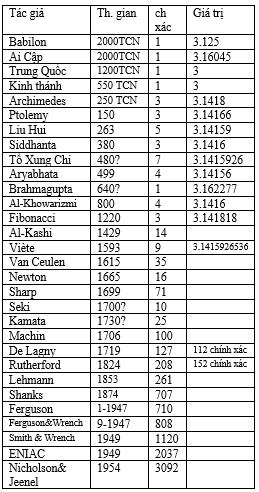
\includegraphics[width= 1\linewidth]{4}
%		\caption{\small\textit{\color{}}}
		\vspace*{-10pt}
	\end{figure}
%%	\vskip 0.1cm
%%	\begin{tabular}{|l|c|c|l}
%%		\hline
%%		Tác giả &	Th. gian&	chuẩn xác&	Giá trị\\
%%		\hline
%%		Babilon&	$2000$TCN&	$1$&	$3.125$\\
%%		\hline
%%		Ai Cập& 	$2000$TCN&	$1$&	$3.16045$\\
%%		\hline
%%		Trung Quốc&	$1200$TCN&	$1$&	$3$\\
%%		\hline
%%		Kinh thánh&	$550$ TCN&	$1$&	$3$\\
%%		\hline
%%		Archimedes&	$250$ TCN&	$3$&	$3.1418$\\
%%		\hline
%%		Ptolemy	&$150$&	$3$&	$3.14166$\\
%%		\hline
%%		Liu Hui	&$263$&	$5$&	$3.14159$\\
%%		\hline
%%		Siddhanta&	$380$&	$3$&	$3.1416$\\
%%		\hline
%%		Tổ Xung Chi&	$480?$&	$7$&	$3.1415926$\\
%%		\hline
%%		Aryabhata&	$499$&	$4$&	$3.14156$\\
%%		\hline
%%		Brahmagupta&	$640?$&	$1$&	$3.162277$\\
%%		\hline
%%		Al--Khowarizmi&	$800$&	$4$&	$3.1416$\\
%%		\hline
%%		Fibonacci&	$1220$&	$3$&	$3.141818$\\
%%		\hline
%%		Al--Kashi&	$1429$&	$14$& \\
%%		\hline
%%		Viète	&$1593$	&$9$&	$3.1415926536$\\
%%		\hline
%%		Van Ceulen&	$1615$&	$35$& \\
%%		\hline	
%%		Newton	&$1665$&	$16$& \\
%%		\hline	
%%		Sharp&	$1699$&	$71$ &	\\
%%		\hline
%%		Seki&	$1700?$&	$10$ &	\\
%%		\hline
%%		Kamata &	$1730?$&	$25$& \\
%%		\hline	
%%		Machin&	$1706$&	$100$& \\
%%		\hline	
%%		De Lagny&	$1719$& $127$&	$112$\\
%%		\hline
%%		Rutherford&	$1824$&	$208$&	$152$\\
%%		\hline
%%		Lehmann&	$1853$&	$261$& \\
%%		\hline	
%%		Shanks&	$1874$&	$707$ & \\
%%		\hline	
%%		Ferguson&	$1-1947$&	$710$ & \\
%%		\hline	
%%		Ferguson\&Wrench&	$9-1947$&	$808$ & \\
%%		\hline 	
%%		Smith \& Wrench&	$1949$& $1120$& \\
%%		\hline 	
%%		ENIAC&	$1949$&	$2037$& \\
%%		\hline	
%%		Nicholson\& Jeenel	&$1954$&$3092$ & \\
%%		\hline	
%%	\end{tabular}
	\textbf{\color{lichsutoanhoc}Phụ lục $\pmb{2}$ Mốc thời gian tính số}  ([$3$], tiếp)
	\begin{figure}[H]
		\vspace*{-5pt}
		\centering
		\captionsetup{labelformat= empty, justification=centering}
		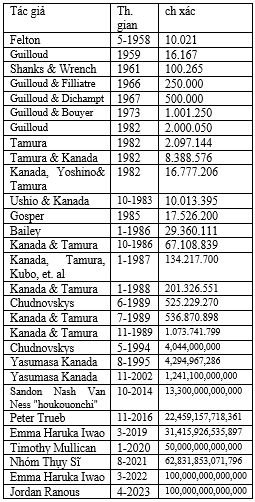
\includegraphics[width= 1\linewidth]{5}
%		\caption{\small\textit{\color{}}}
		\vspace*{-10pt}
	\end{figure}
%	\begin{tabular}{|l|c|c|l|}
%		\hline
%		Tác giả& 	Th. gian&	ch xác
%		Felton	5-1958	10.021
%		Guilloud	1959	16.167
%		Shanks & Wrench	1961	100.265
%		Guilloud & Filliatre	1966	250.000
%		Guilloud & Dichampt	1967	500.000
%		Guilloud & Bouyer	1973	1.001.250
%		Guilloud	1982	2.000.050
%		Tamura	1982	2.097.144
%		Tamura & Kanada	1982	8.388.576
%		Kanada, Yoshino& Tamura	1982	16.777.206
%		Ushio & Kanada	10-1983	10.013.395
%		Gosper	1985	17.526.200
%		Bailey	1-1986	29.360.111
%		Kanada & Tamura	10-1986	67.108.839
%		Kanada, Tamura, Kubo, et. al	1-1987	134.217.700
%		Kanada & Tamura	1-1988	201.326.551
%		Chudnovskys	6-1989	525.229.270
%		Kanada & Tamura	7-1989	536.870.898
%		Kanada & Tamura	11-1989	1.073.741.799
%		Chudnovskys	5-1994	4,044,000,000
%		Yasumasa Kanada	8-1995	4,294,967,286
%		Yasumasa Kanada	11-2002	1,241,100,000,000
%		Sandon Nash Van Ness "houkouonchi"	10-2014	13,300,000,000,000
%		Peter Trueb	11-2016	22,459,157,718,361
%		Emma Haruka Iwao
%		3-2019	31,415,926,535,897
%		Timothy Mullican	1-2020	50,000,000,000,000
%		Nhóm Thụy Sĩ	8-2021	62,831,853,071,796
%		Emma Haruka Iwao
%		3-2022	100,000,000,000,000
%		Jordan Ranous	4-2023	100,000,000,000,000
%	\end{tabular}
	\textbf{\color{lichsutoanhoc}Phụ lục $\pmb{3}$ Thực hành tính số $\pmb{\pi}$  với GeoGebra}
	\vskip 0.1cm
	Phụ lục này giới thiệu cách tính số $\pi$ trên \textit{GeoGebra} có thể phục vụ trong dạy và học.
	\vskip 0.1cm
	\textbf{\color{lichsutoanhoc}Thuật toán tính số Pi theo chuỗi} Trong \textit{GeoGebra}, việc tính xấp xỉ số $\pi$ dựa theo các công thức dạng chuỗi là tương đối thuận tiện. Ví dụ, với công thức của Euler ($9$) cho $\frac{n^2}{6}$, ta tính tổng của chuỗi theo lệnh sau:
	\begin{align*}
		s = Sum\left( {Sequence\left( {\frac{1}{{{a^2}}},a,1,n} \right)} \right)
	\end{align*}
	với $n$ là giá trị cho trước. Ở đây lệnh \textit{Sequence} sẽ tạo ra một dãy số có các phần tử là $\frac{1}{a^2}$ với  $1 \le a \le n$. Giá trị của $\pi$  có thể được tính bằng $\sqrt{6s}$. Với giá trị $n$ càng lớn thì giá trị của $\pi$  càng chính xác hơn. Chẳng hạn, với $n = 10^6$  lệnh
	\begin{align*}
		s = Sum\left( {Sequence\left( {\frac{1}{{{a^2}}},a,1,10\^6} \right)} \right)
	\end{align*}
	cho $\pi \approx 3.14159$ (tính toán này mất khoảng vài phút trong \textit{GeoGebra}). Các công thức khác dạng chuỗi của Euler hay của Ramanujan hoặc Comtet đều có thể tính theo phương pháp trên trong \textit{GeoGebra}.
	\vskip 0.1cm
	Với công thức Gregory -- Leibnitz hoặc các công thức dạng Machin, các số hạng của chuỗi liên quan đến các số lẻ và dấu được đảo liên tiếp. Biểu thức tính dấu của mỗi số hạng sẽ tương đối phức tạp. Tuy nhiên, ta có thể sử dụng mẹo đặt bước của dãy số là 4 và sinh hai thay vì chỉ một số hạng ở mỗi bước. Ví dụ với công thức Gregory-Leibnitz ta làm như sau:
	\begin{align*}
		4*Sum\!\!\left(\!\! {Sequence\left(\!\! {\frac{1}{a}\! -\! \frac{1}{{a \!+\! 2}},a,1,n \!+\! 1,4} \!\!\right)}\!\! \right)
	\end{align*}
	với $n$ là một số chia hết cho $4$. Các số hạng sẽ được sinh theo cặp:$1 - \frac{1}{3}m \frac{1}{5} - \frac{1}{7}, \ldots$.
	\vskip 0.1cm  
	Với  $n = 10^6$, ta thu được giá trị của $\pi$  là $3.14159$. Bạn đọc có thể tự sử dụng cách này để tính  $\pi$  theo các công thức dạng Machin.
	\vskip 0.1cm
	\textbf{\color{lichsutoanhoc}Tính số Pi trên GeoGebra theo Archimedes}
	\vskip 0.1cm 
	Có thể sử dụng \textit{GeoGebra} để minh họa cách tính số $\pi$  theo thuật toán Archimedes như sau. Thiết lập các đường tròn cùng với các đa giác đều nội ngoại tiếp theo các bước sau. Cũng có thể sử dụng các file .ggb \textit{GeoGebra} có sẵn trên mạng.  
	\vskip 0.1cm
	\textbf{\color{lichsutoanhoc}Bước} $\pmb1$: Dùng công cụ vẽ đường tròn 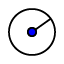
\includegraphics[scale =0.25]{6}: Khai báo tâm (nhấn chuột được một điểm), chọn bán kính $0.5$ (đường kính bằng $1$).
	\vskip 0.1cm 
	\textbf{\color{lichsutoanhoc}Bước} $\pmb{2}$: Phóng to hình cho dễ nhìn đường tròn.
	\vskip 0.1cm
	\textbf{\color{lichsutoanhoc}Bước} $\pmb{3}$: Vẽ đa giác đều nhớ công cụ 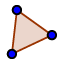
\includegraphics[scale =0.25]{7} đa giác đều (thí dụ, tam giác hoặc tứ giác đều). Nháy vào đỉnh đầu tiên để kết thúc vẽ đa giác đều nội tiếp.
	\vskip 0.1cm
	\textbf{\color{lichsutoanhoc}Bước} $\pmb{4}$: Chọn nút công cụ chuyển động 
\includegraphics[scale =0.25]{8} và vẫn giữ nguyên hình (tam giác hoặc vuông).
	\vskip 0.1cm
	\textbf{\color{lichsutoanhoc}Bước} $\pmb{5}$: Chọn công cụ Khoảng cách hoặc Độ dài.  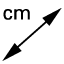
\includegraphics[scale =0.25]{9}. Chọn một điểm bên trong đường tròn nội tiếp để xuất hiện số đo chu vi. Ghi số đo chu vi xuống phía dưới. 
	\vskip 0.1cm
	\textbf{\color{lichsutoanhoc}Bước} $\pmb{6}$: Dùng quy trình trên để vẽ và tìm chu vi đa giác đều $6$ cạnh, $12$ cạnh, $24$, $48$ và $96$ cạnh.
	\vskip 0.1cm
	\textbf{\color{lichsutoanhoc}Bước} $\pmb{7}$: Làm tương tự với đa giác đều ngoại tiếp và so sánh với chu vi đa giác đều nội tiếp và đi đến kết luận xấp xỉ số $\pi$.
	\vskip 0.1cm  
	Dưới đây là một số hình ảnh minh họa. :
	\begin{figure}[H]
		\vspace*{-5pt}
		\centering
		\captionsetup{labelformat= empty, justification=centering}
		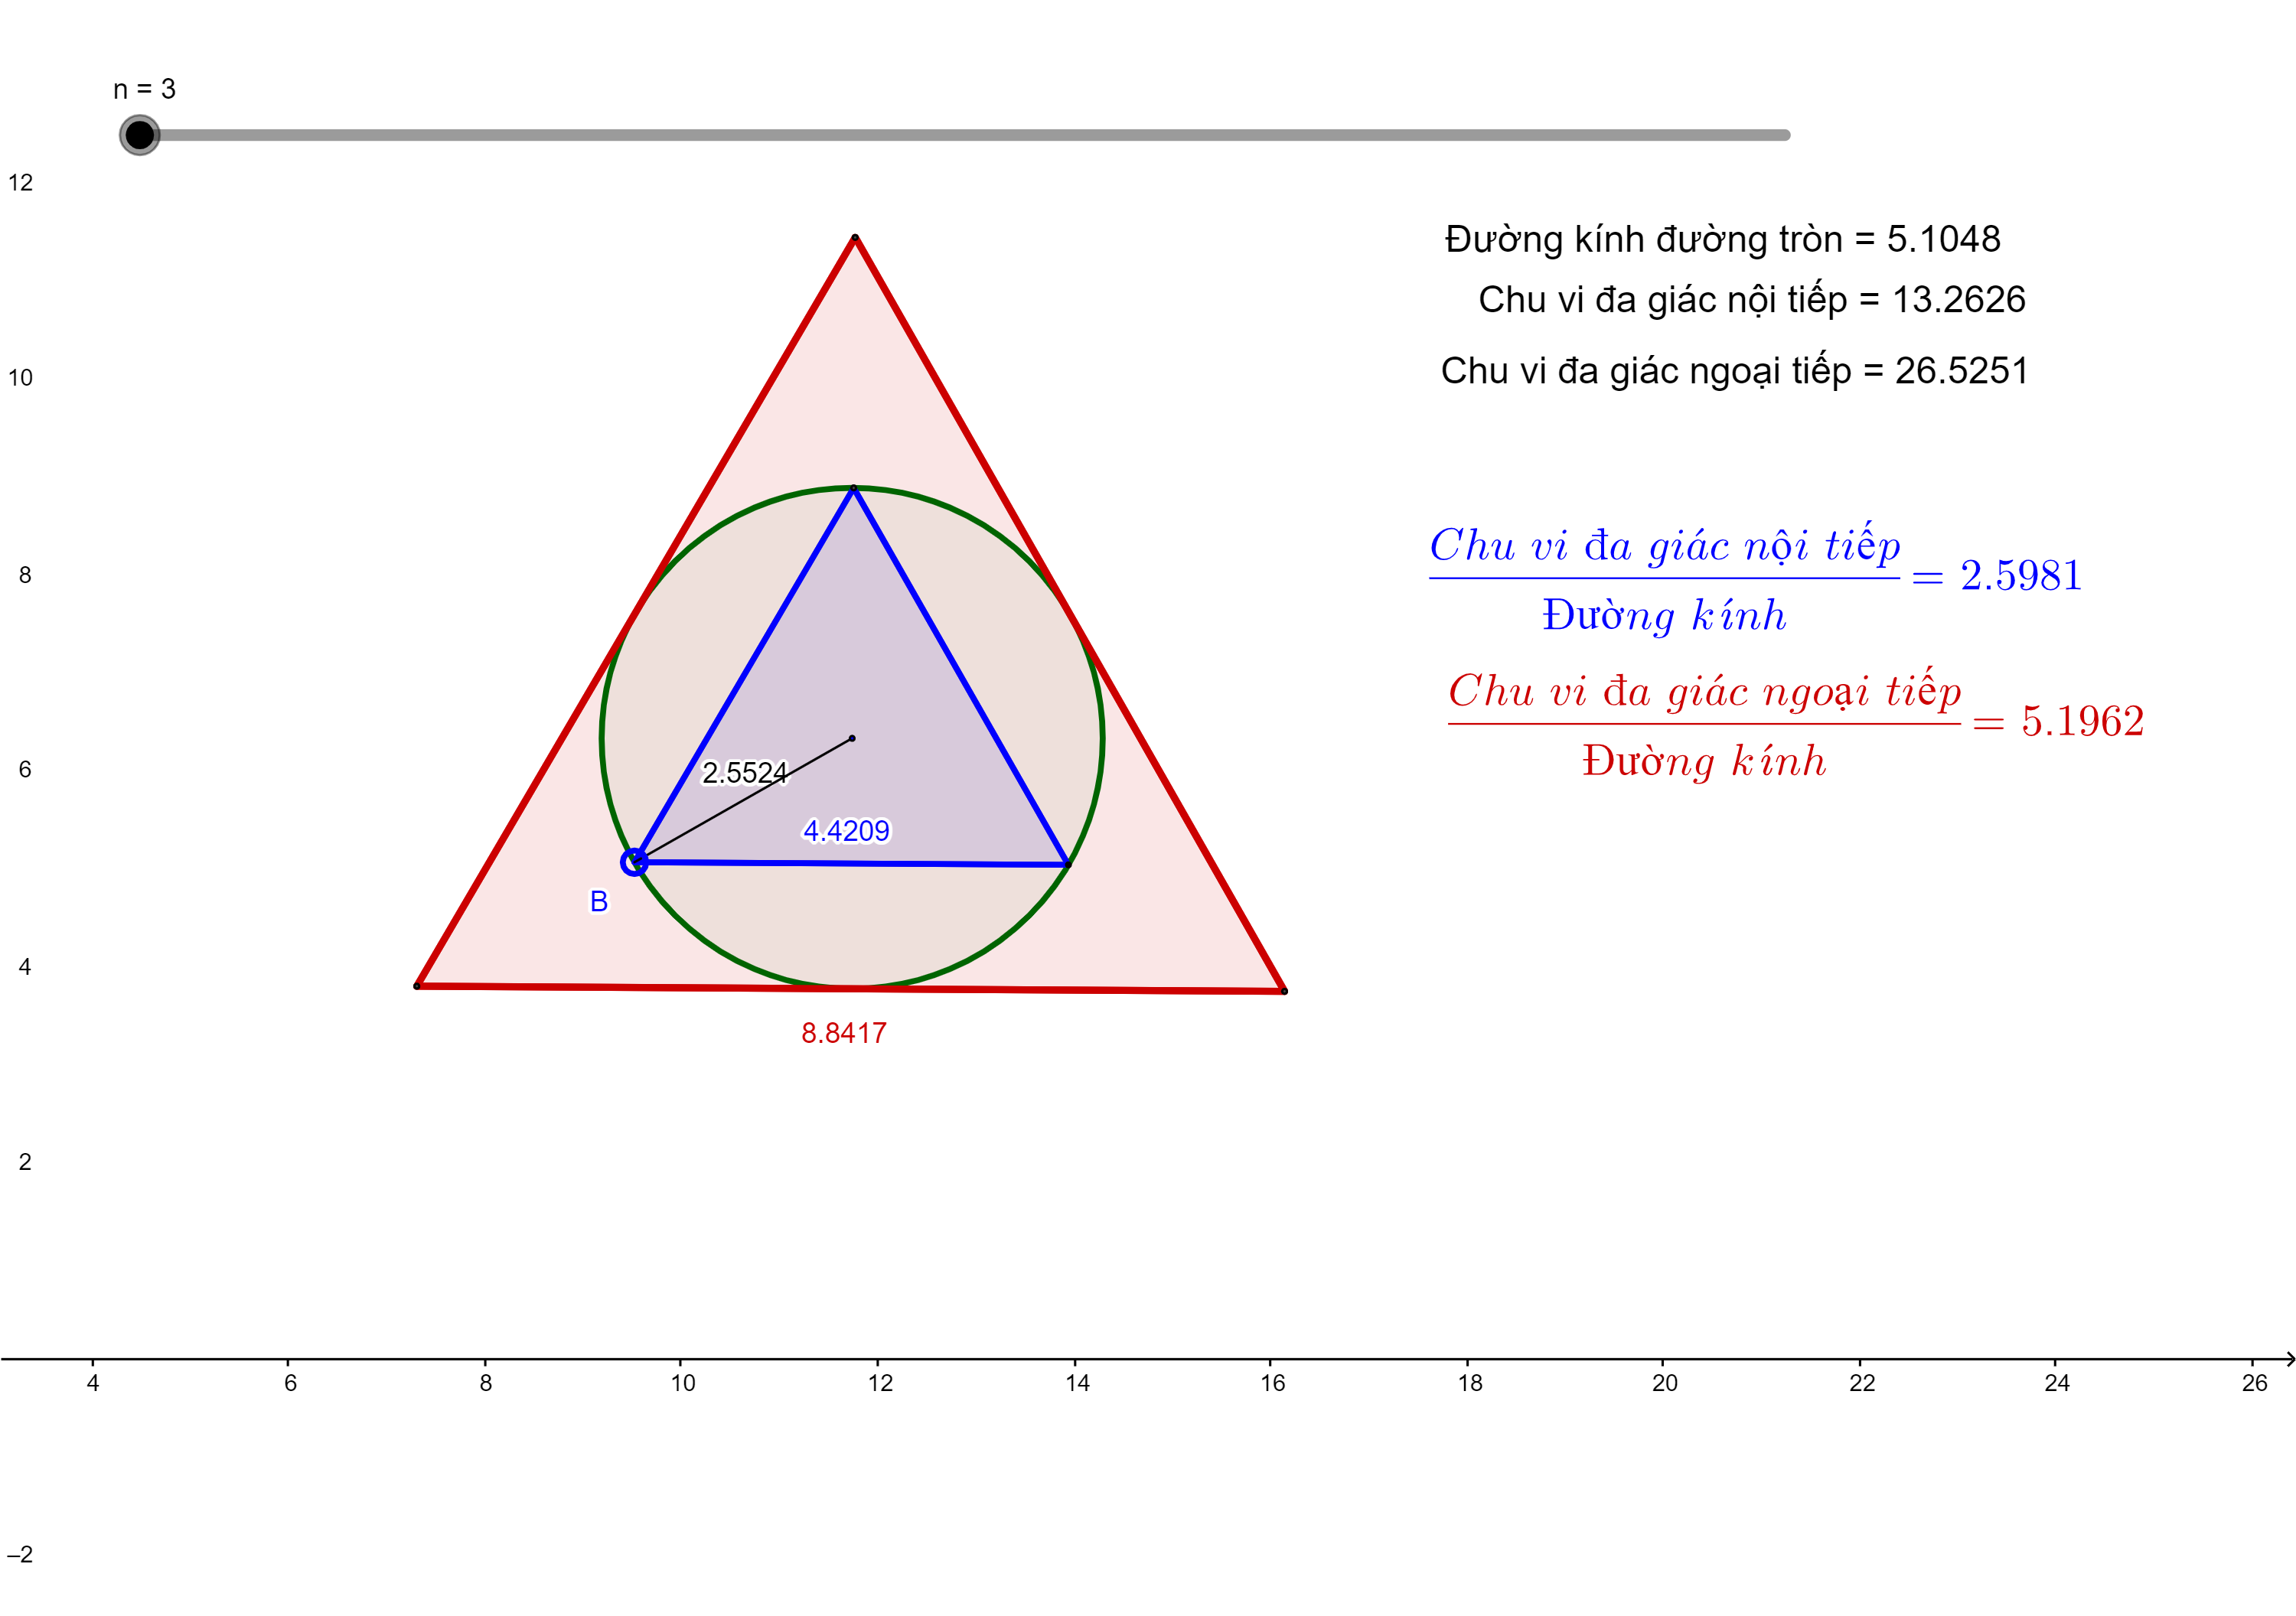
\includegraphics[width= 1\linewidth]{10}
		\caption{\small\textit{\color{lichsutoanhoc}$n = 3$}}
		\vspace*{-10pt}
	\end{figure}
	\begin{figure}[H]
		\vspace*{-5pt}
		\centering
		\captionsetup{labelformat= empty, justification=centering}
		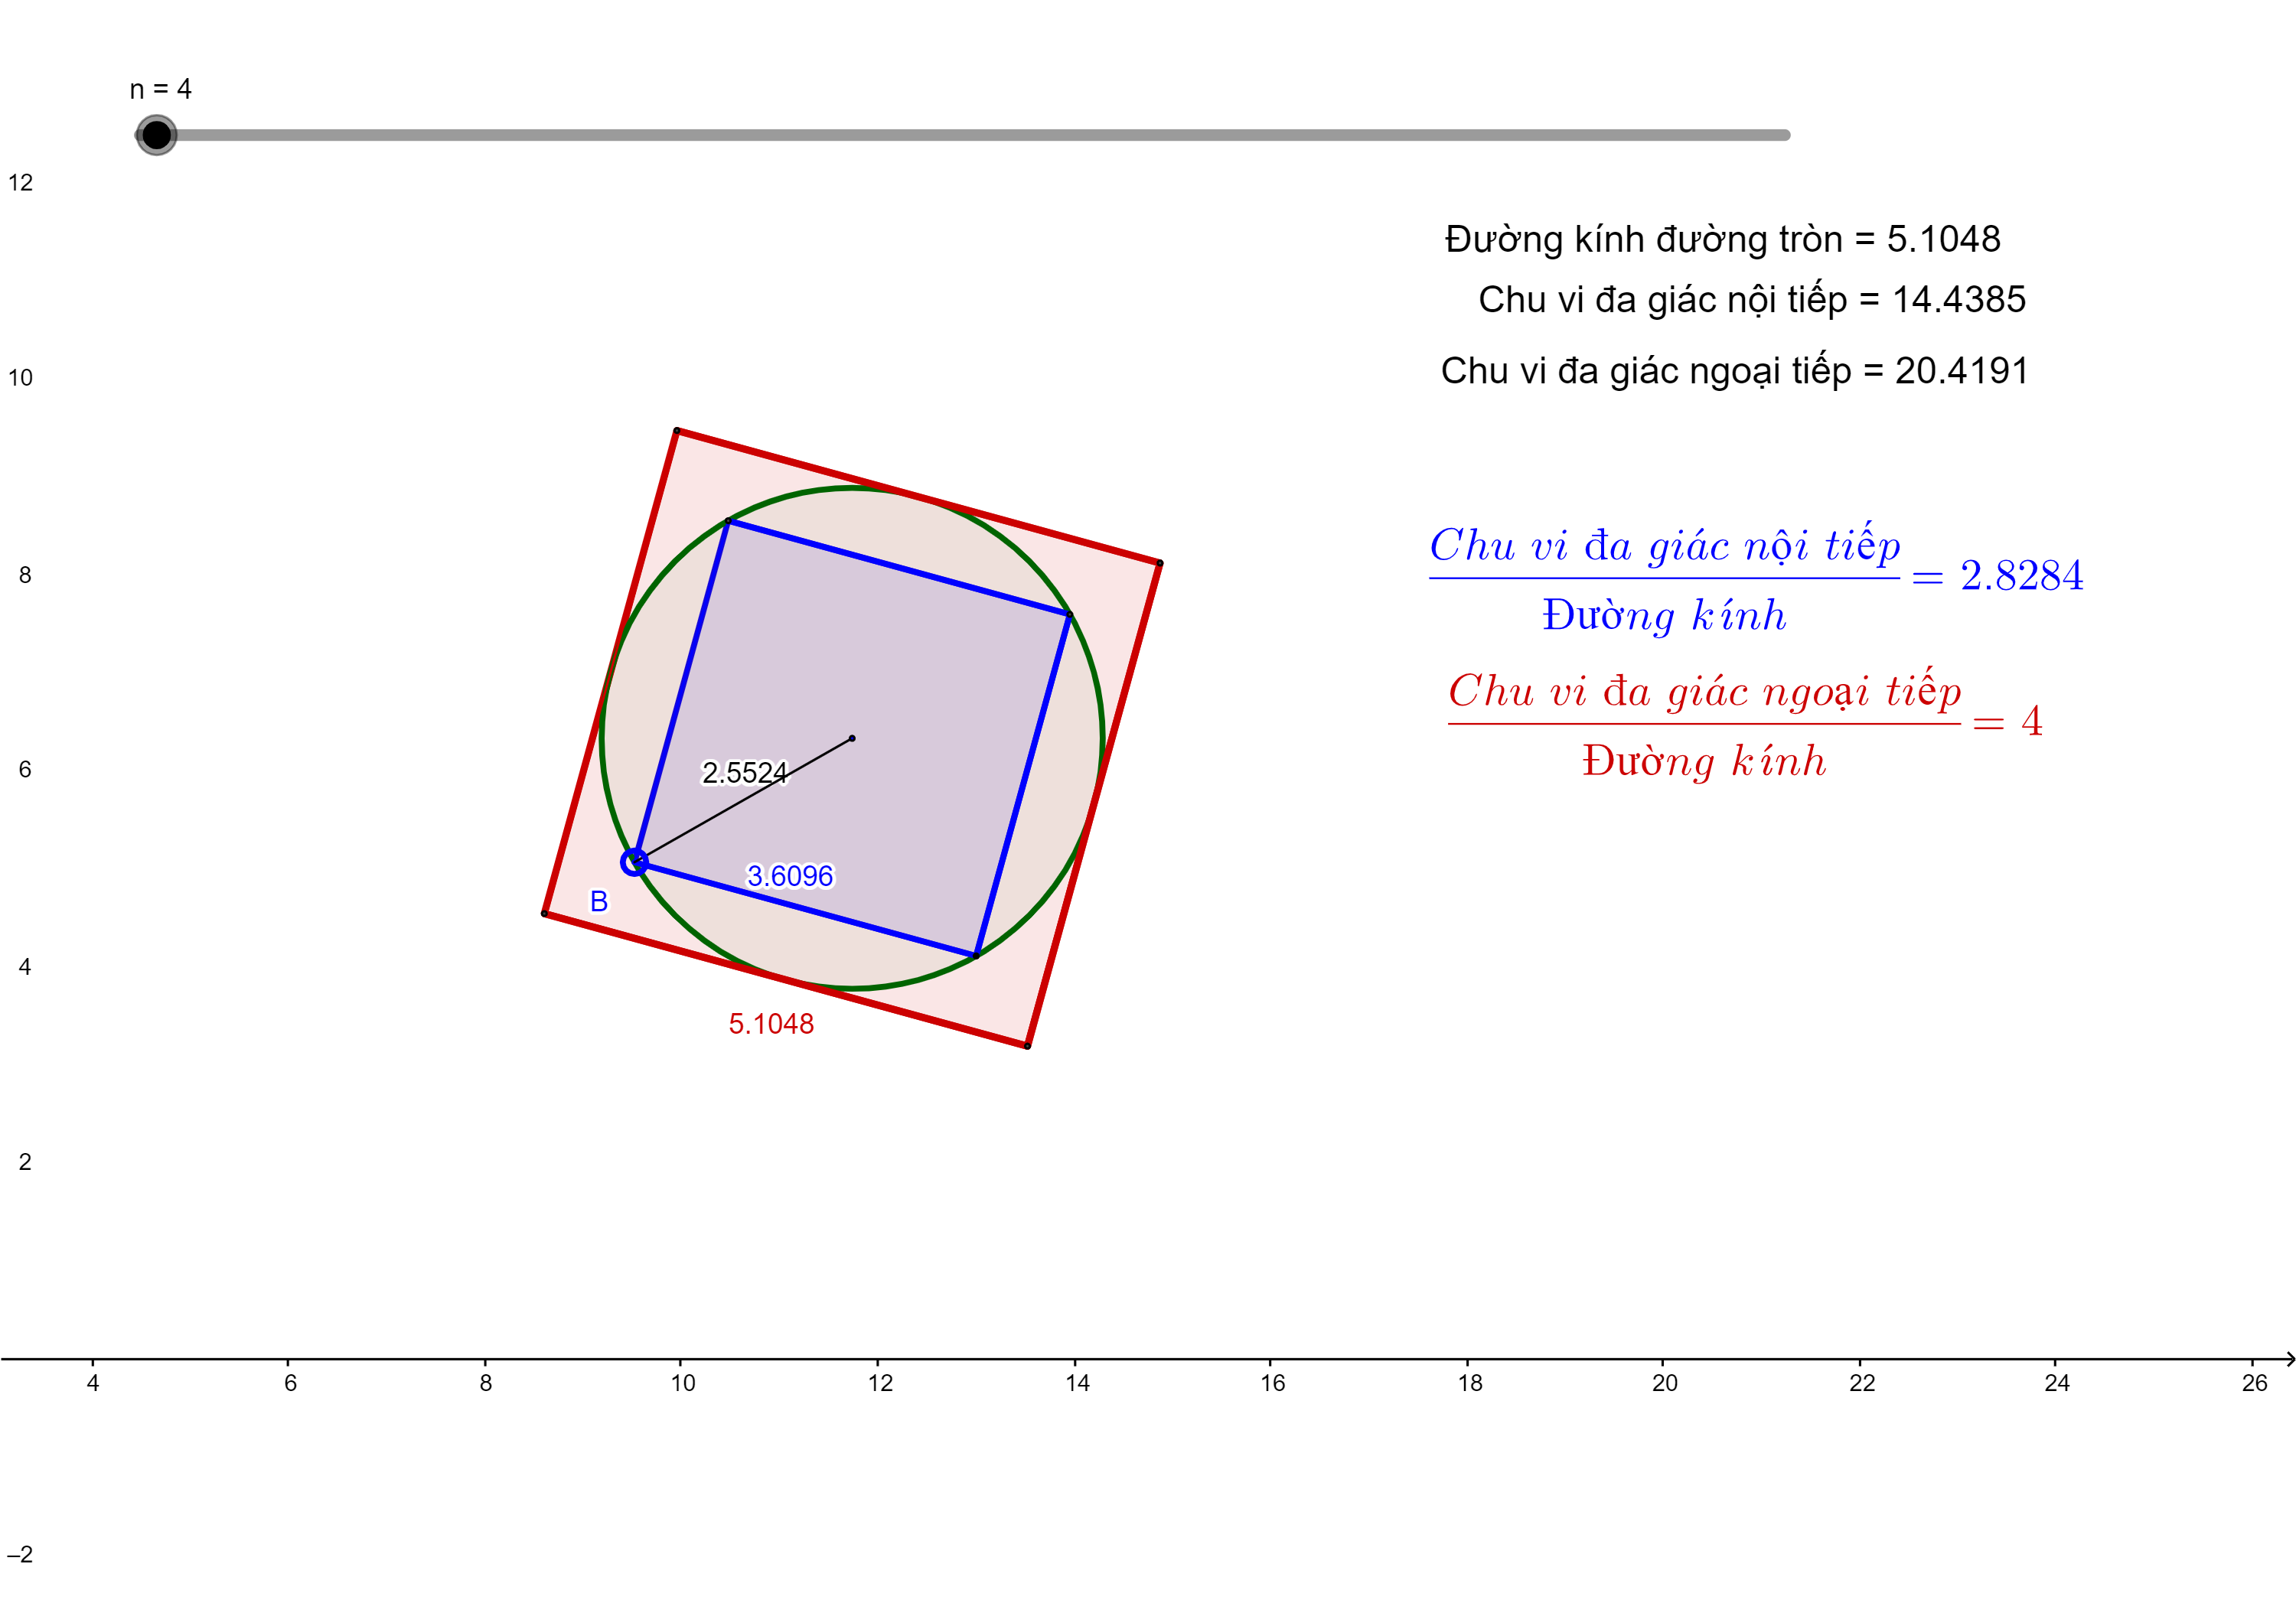
\includegraphics[width= 1\linewidth]{11}
	\caption{\small\textit{\color{lichsutoanhoc}$n = 4$.}}
	\end{figure}
%	\begin{figure}[H]
%		\vspace*{-5pt}
%		\centering
%		\captionsetup{labelformat= empty, justification=centering}
%		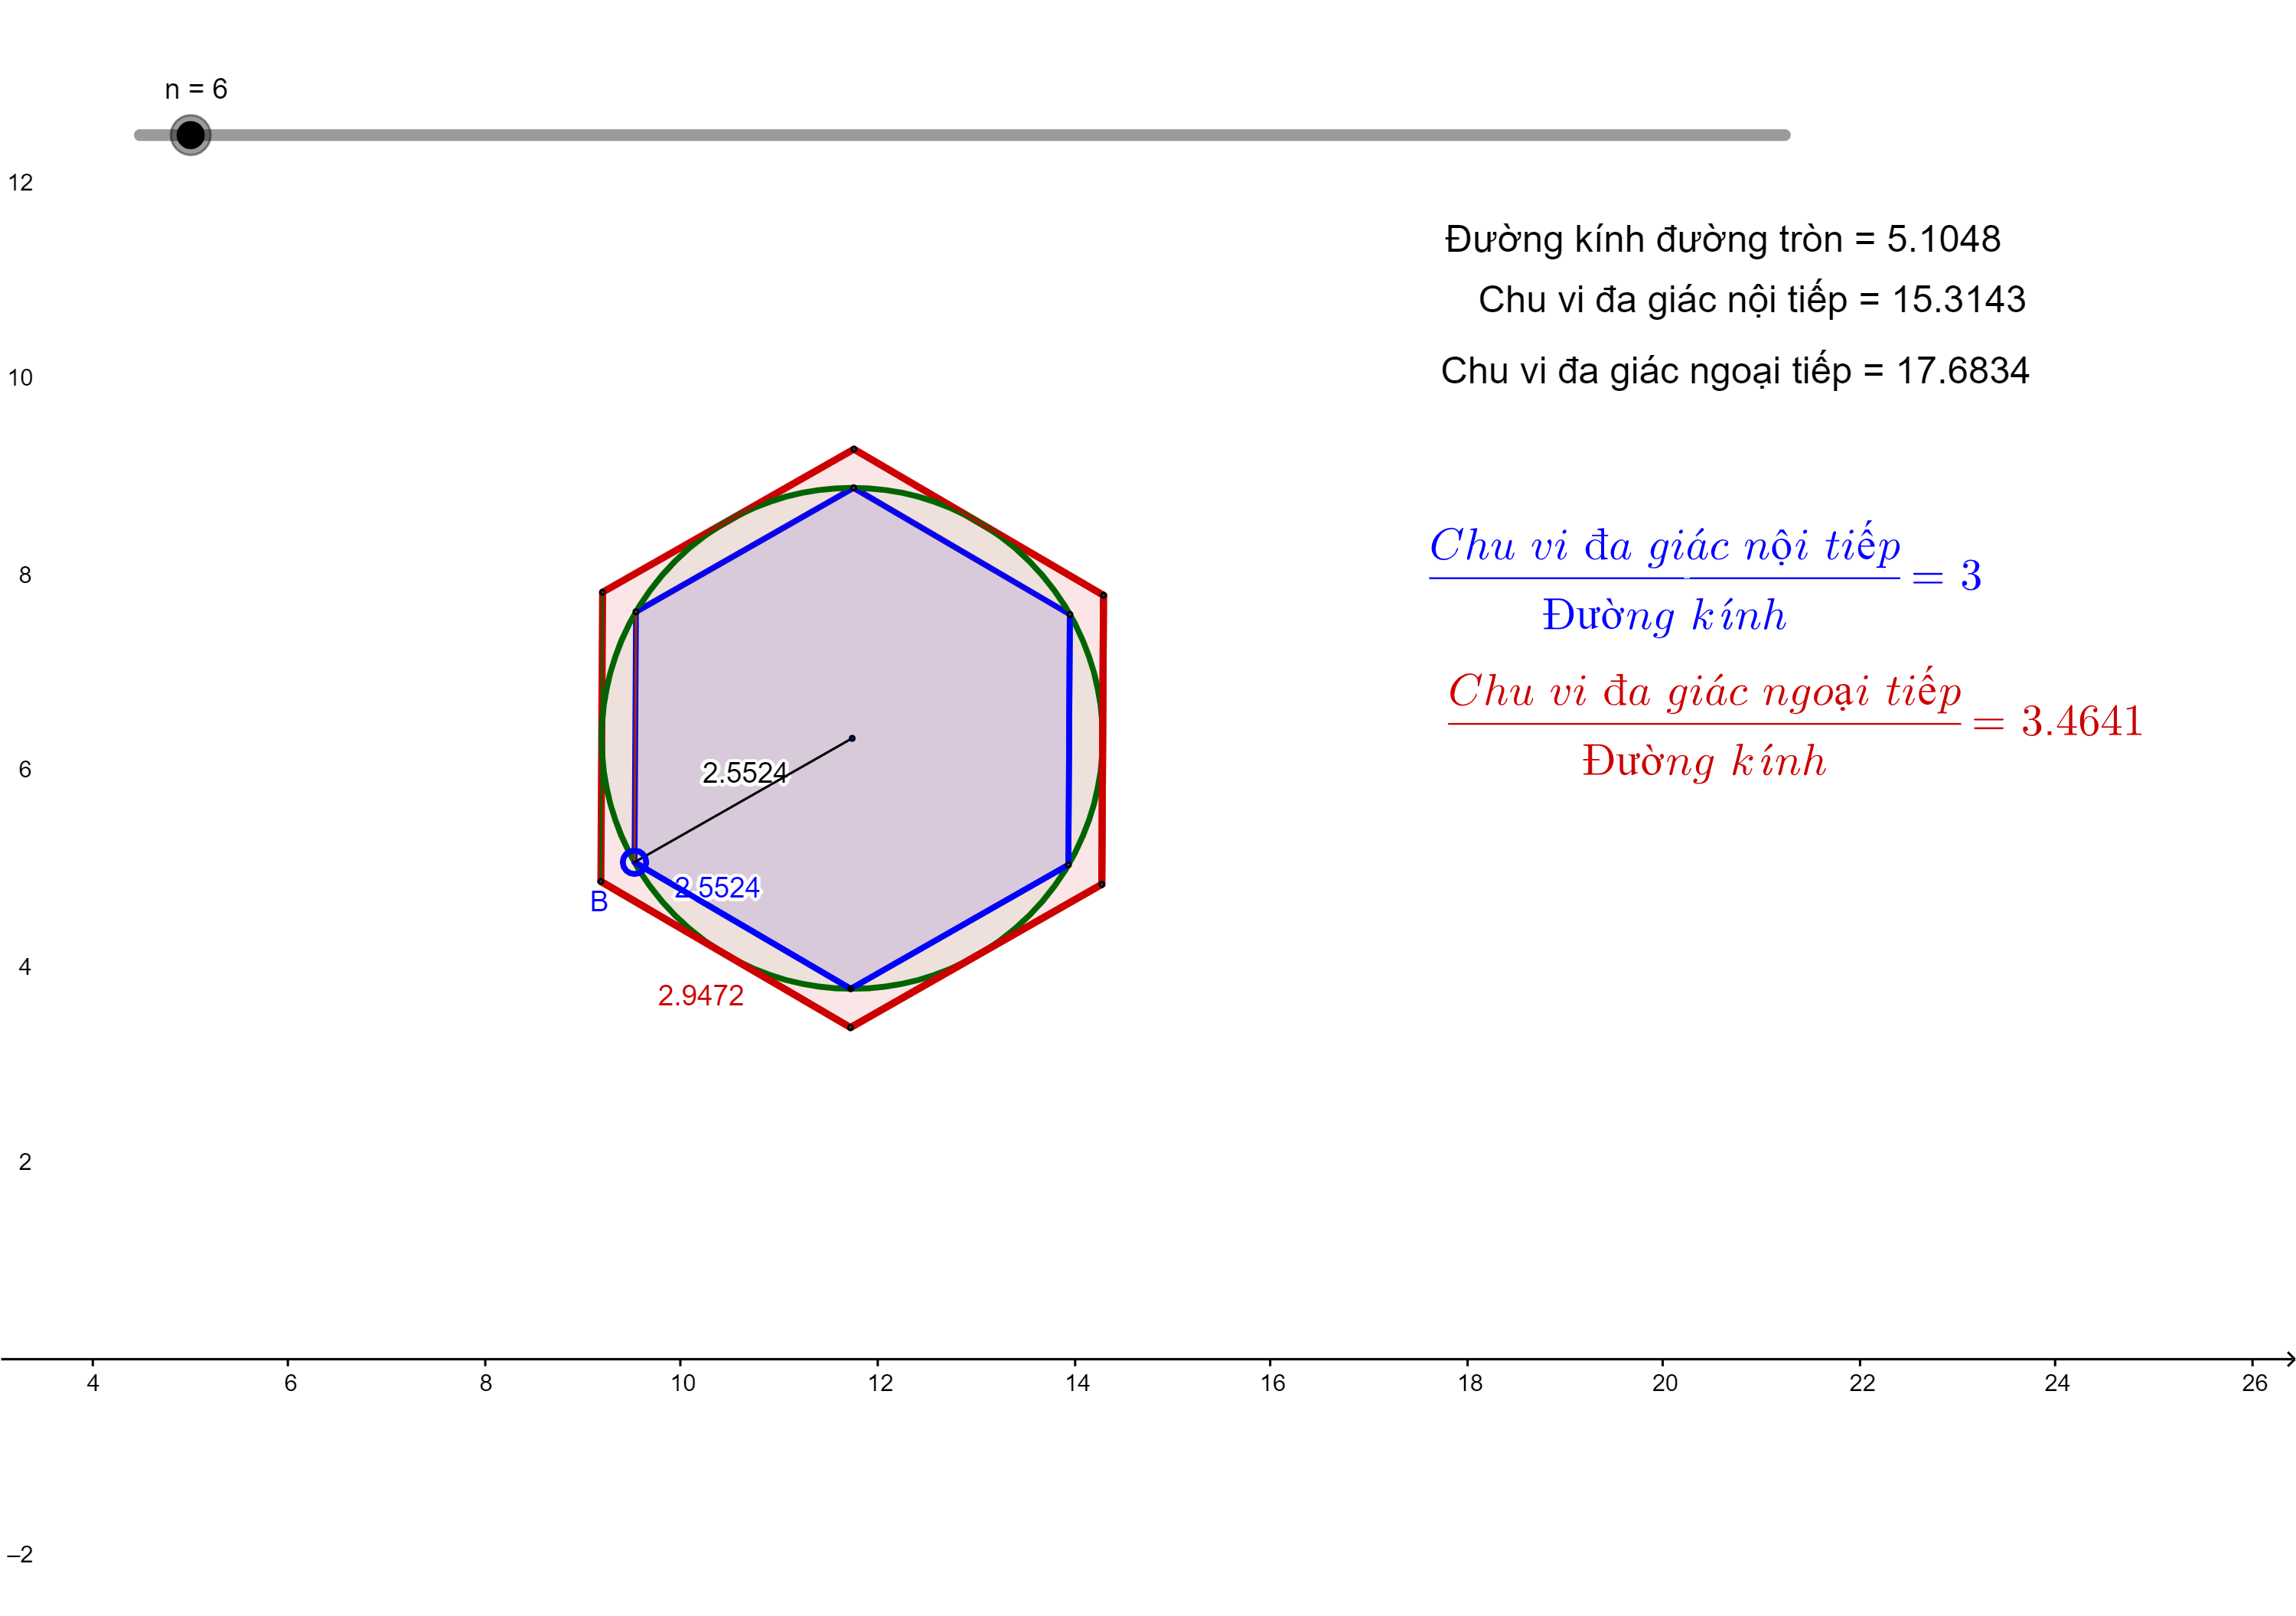
\includegraphics[width= 1\linewidth]{12}
%		\caption{\small\textit{\color{lichsutoanhoc}$n = 6$.}}
%		\vspace*{-10pt}
%	\end{figure}
	\begin{figure}[H]
		\vspace*{-5pt}
		\centering
		\captionsetup{labelformat= empty, justification=centering}
		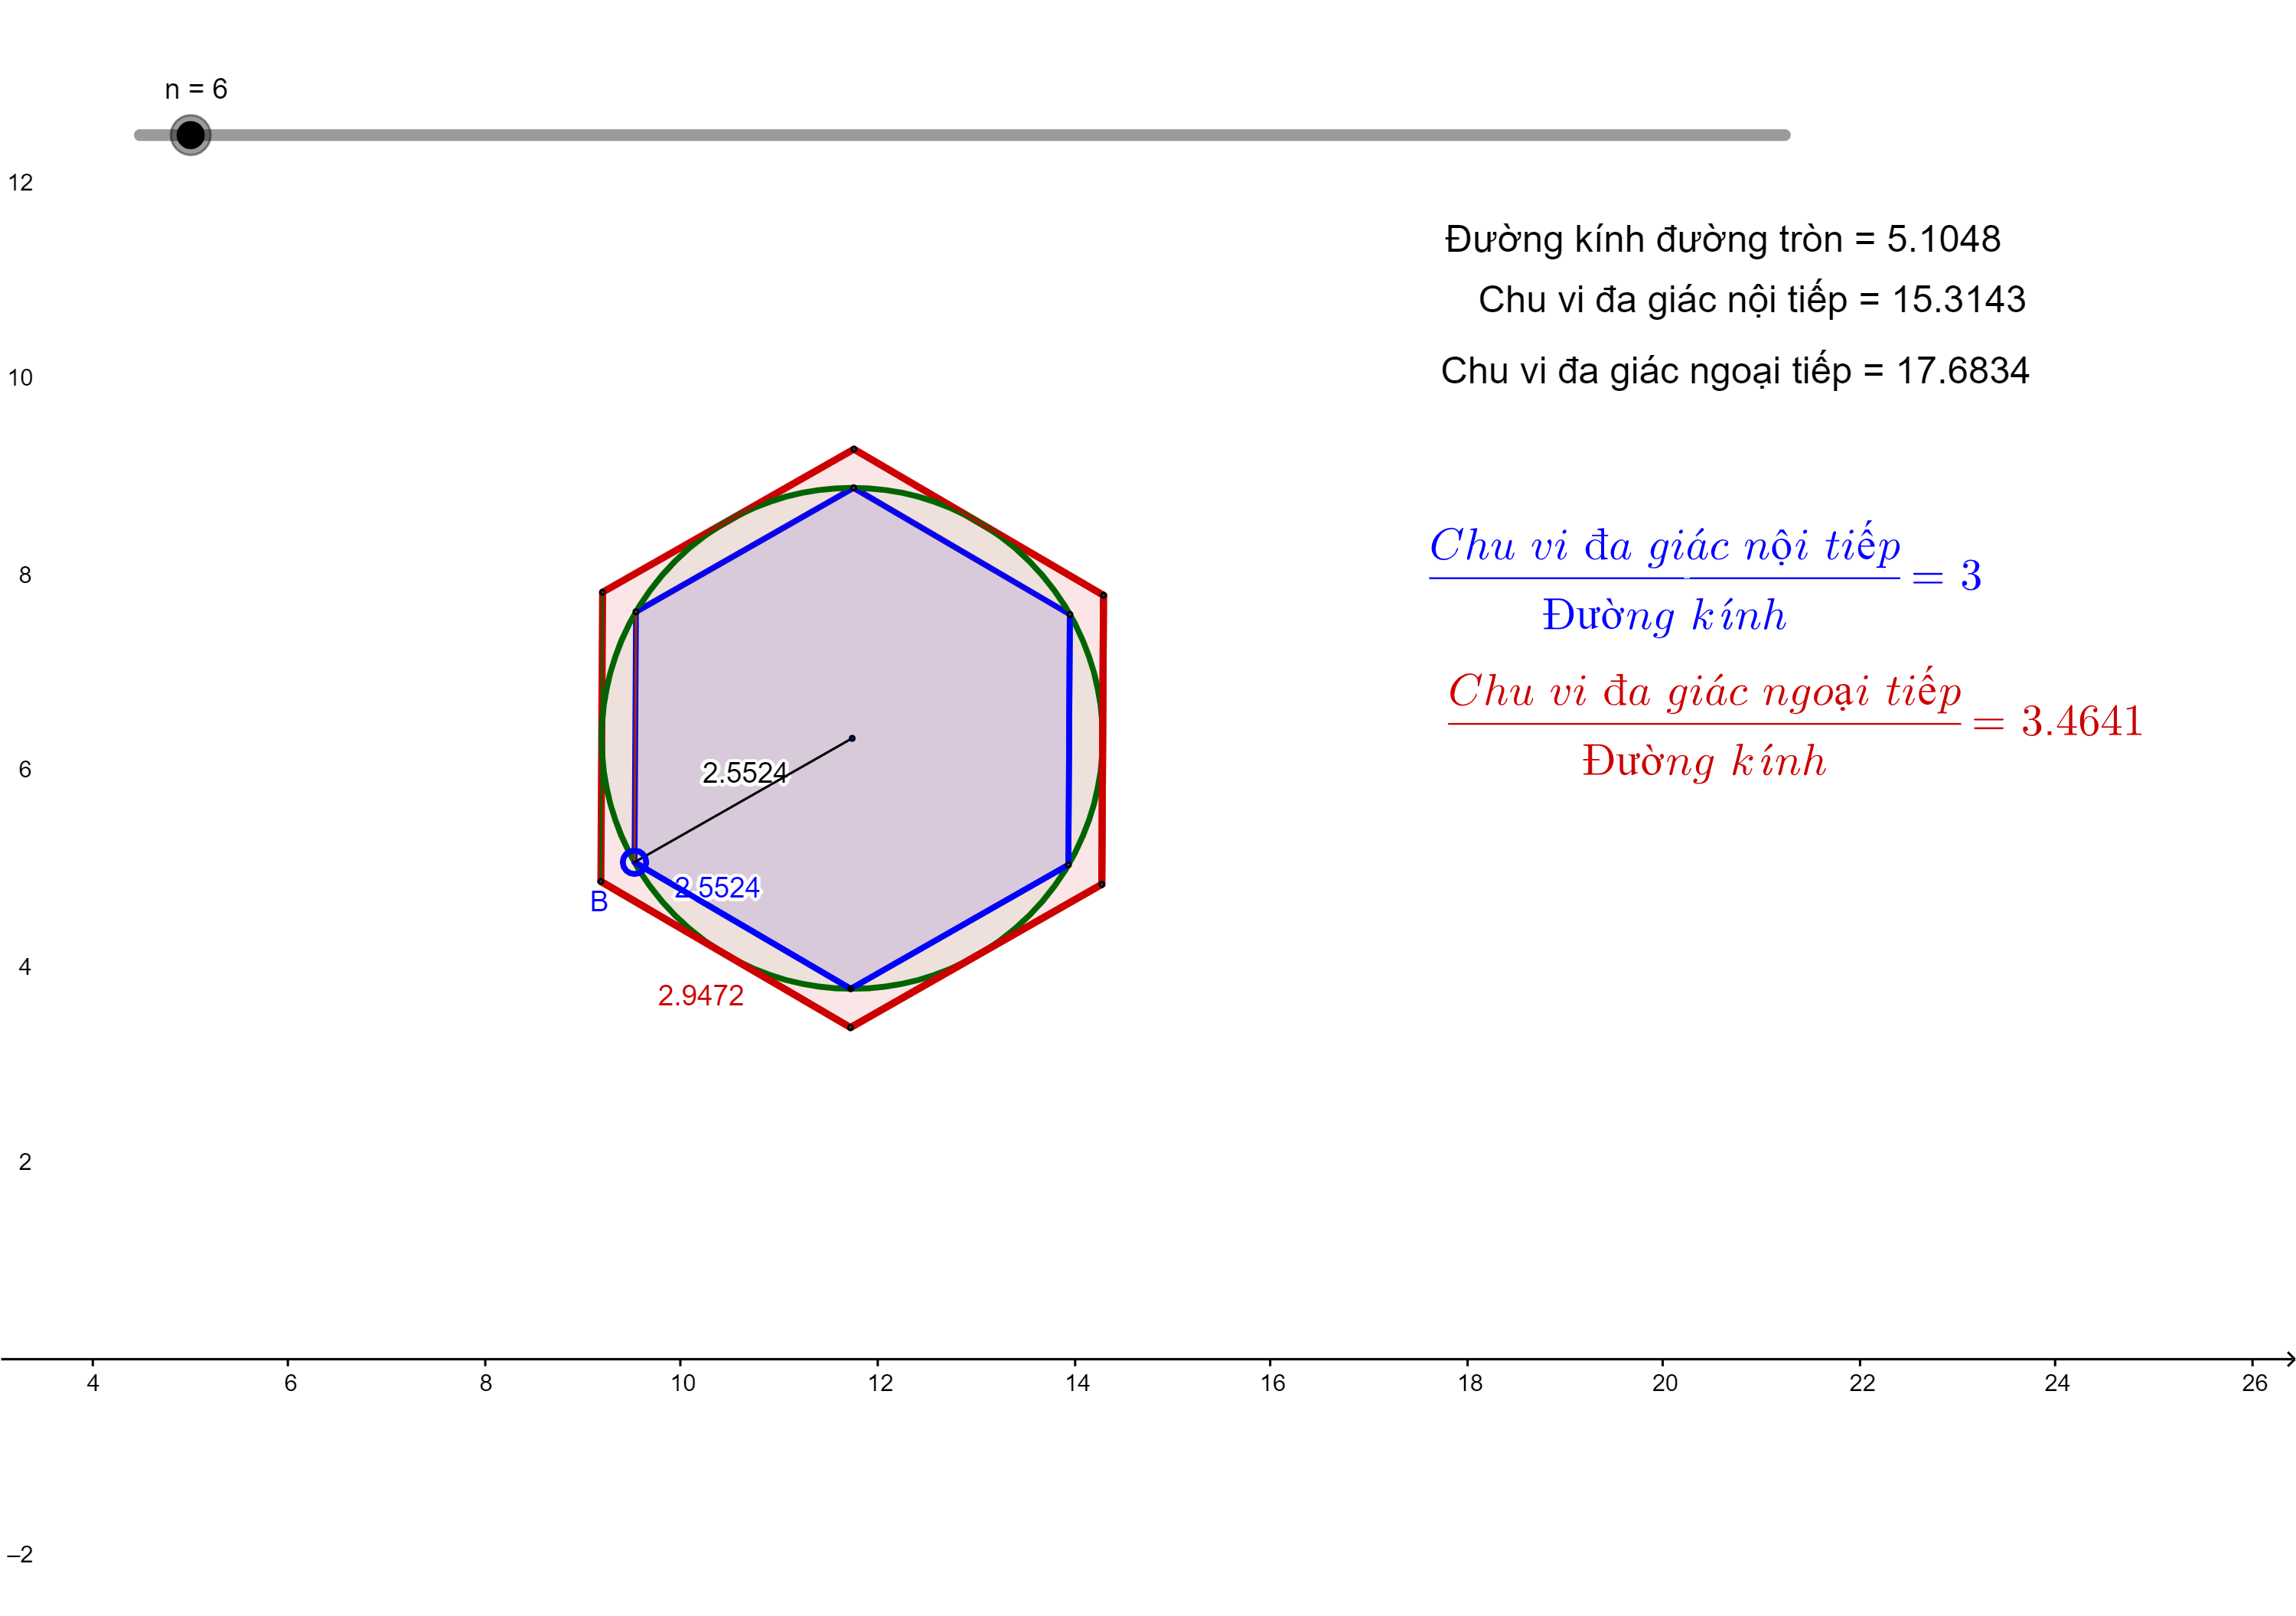
\includegraphics[width= 1\linewidth]{12}
		\caption{\small\textit{\color{lichsutoanhoc}$n = 6$.}}
		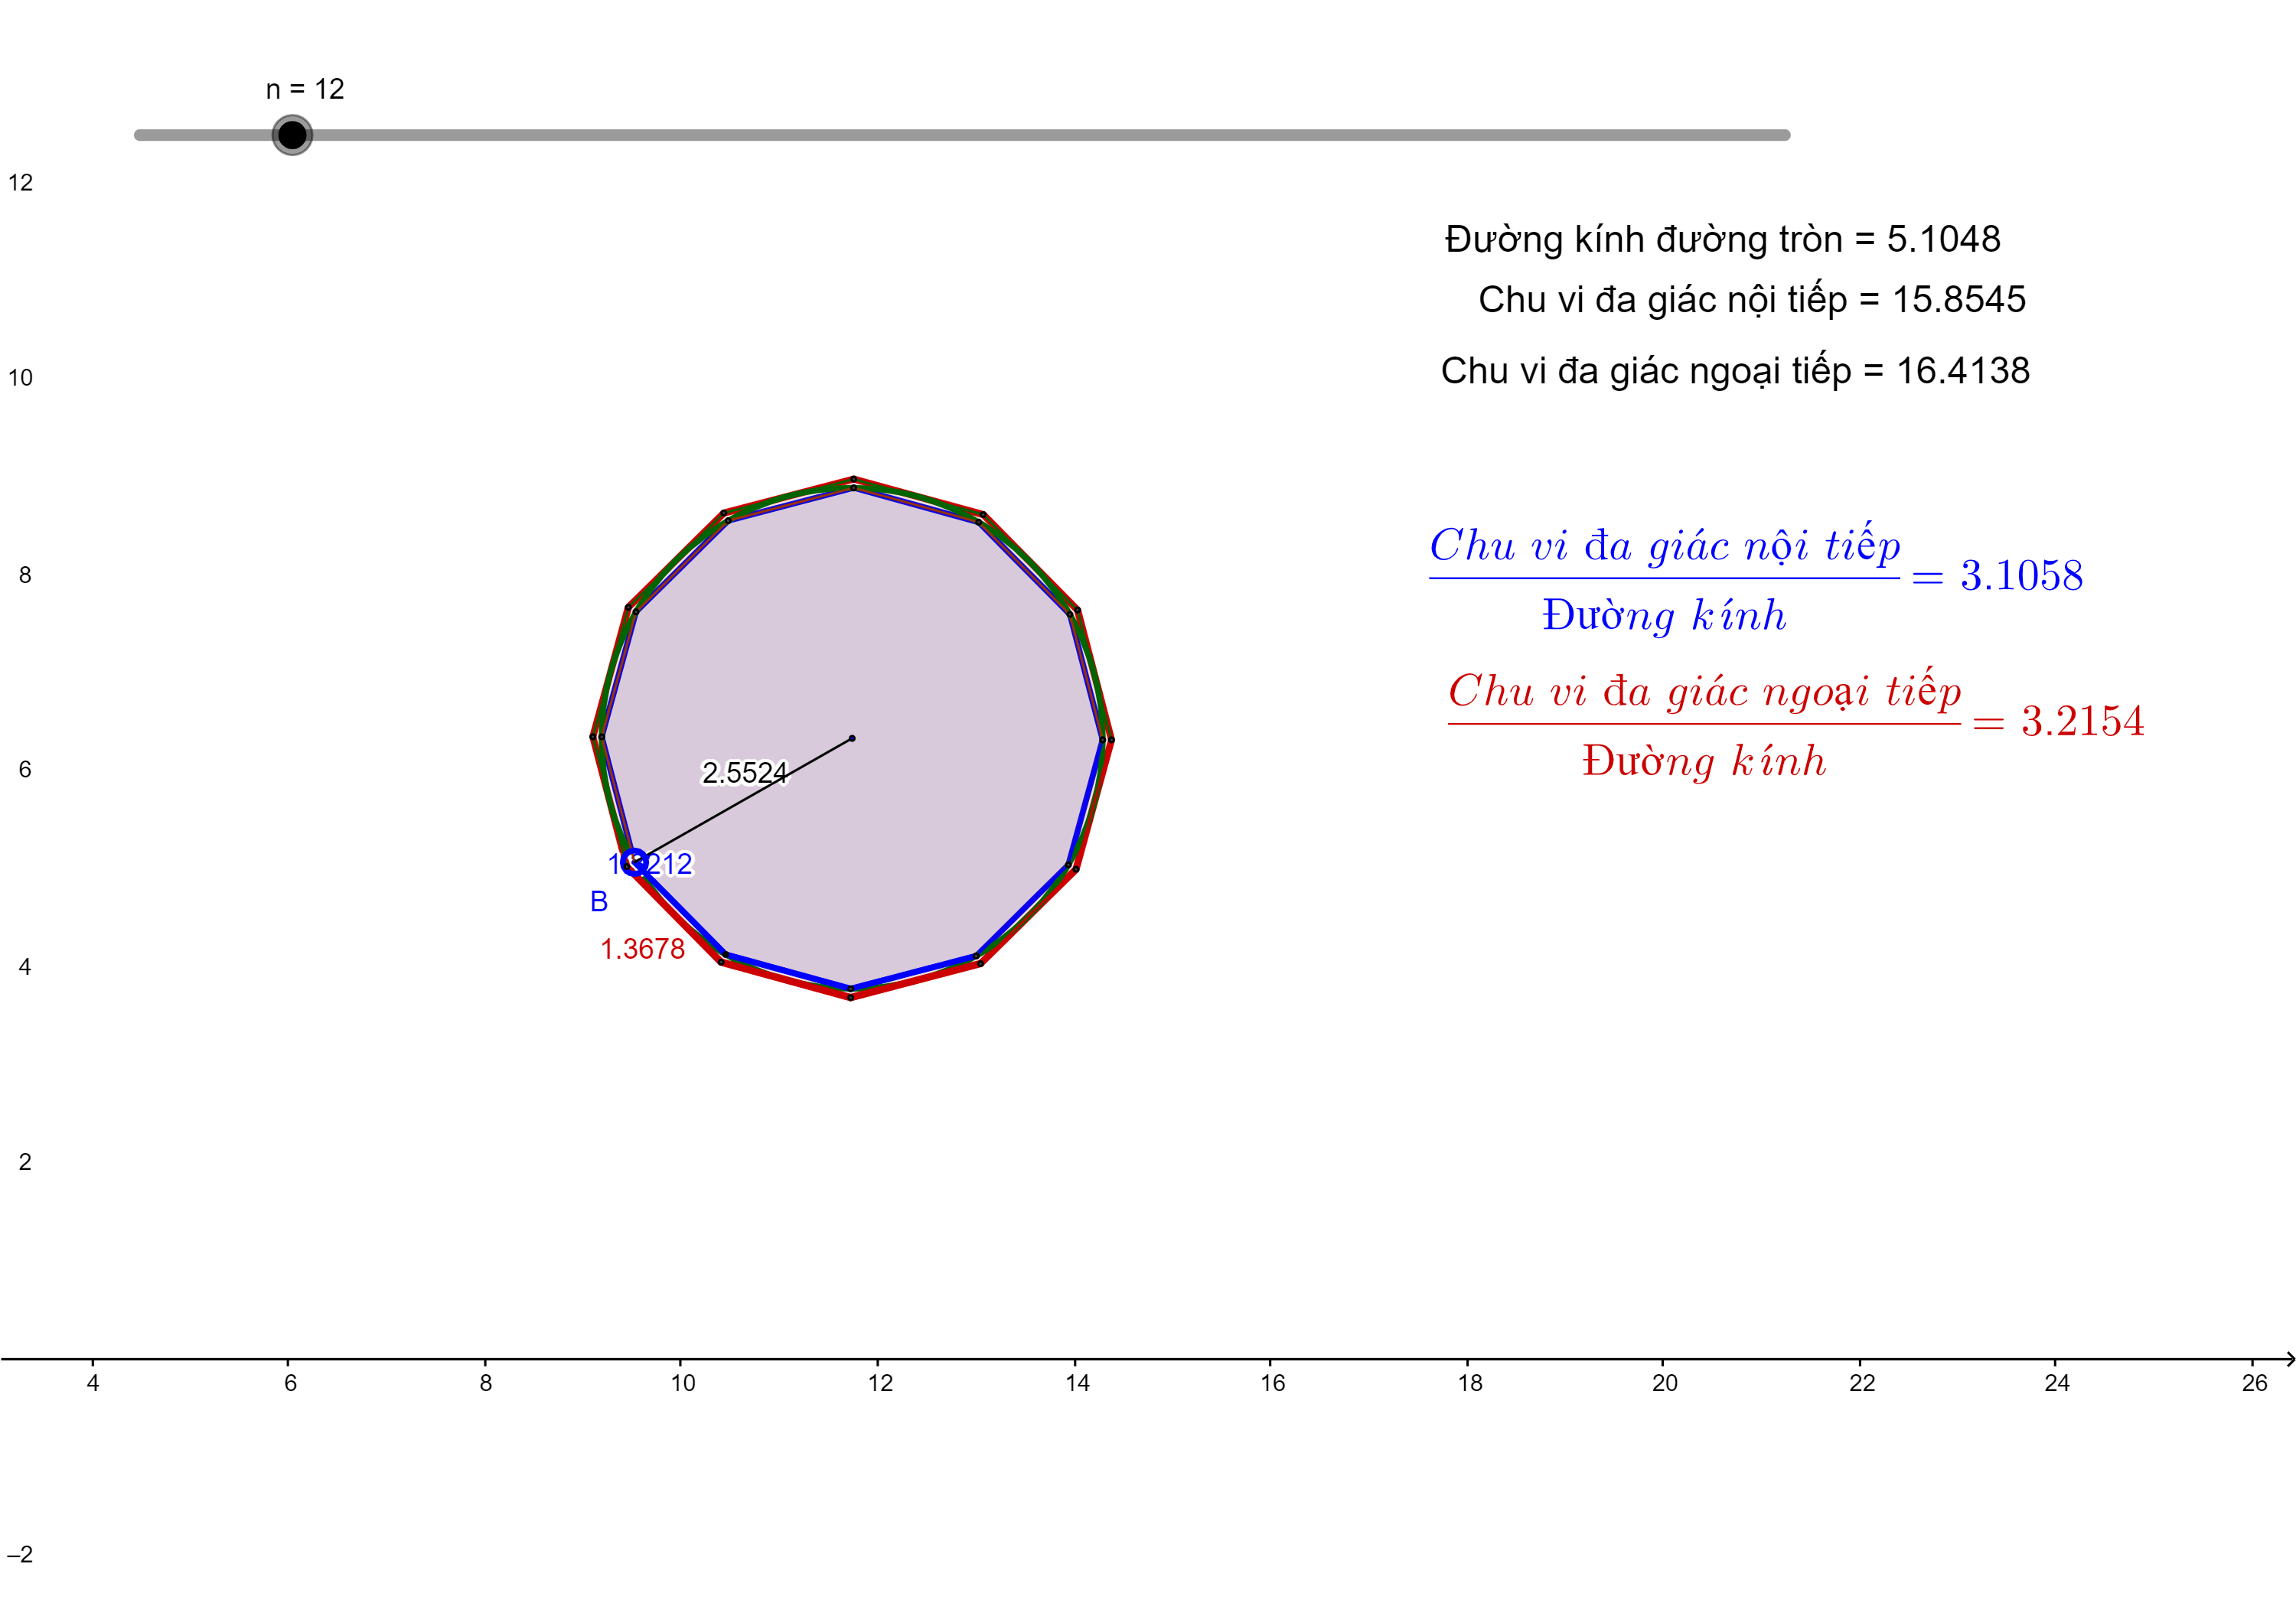
\includegraphics[width= 1\linewidth]{13}
		\caption{\small\textit{\color{lichsutoanhoc}$n = 12$.}}
		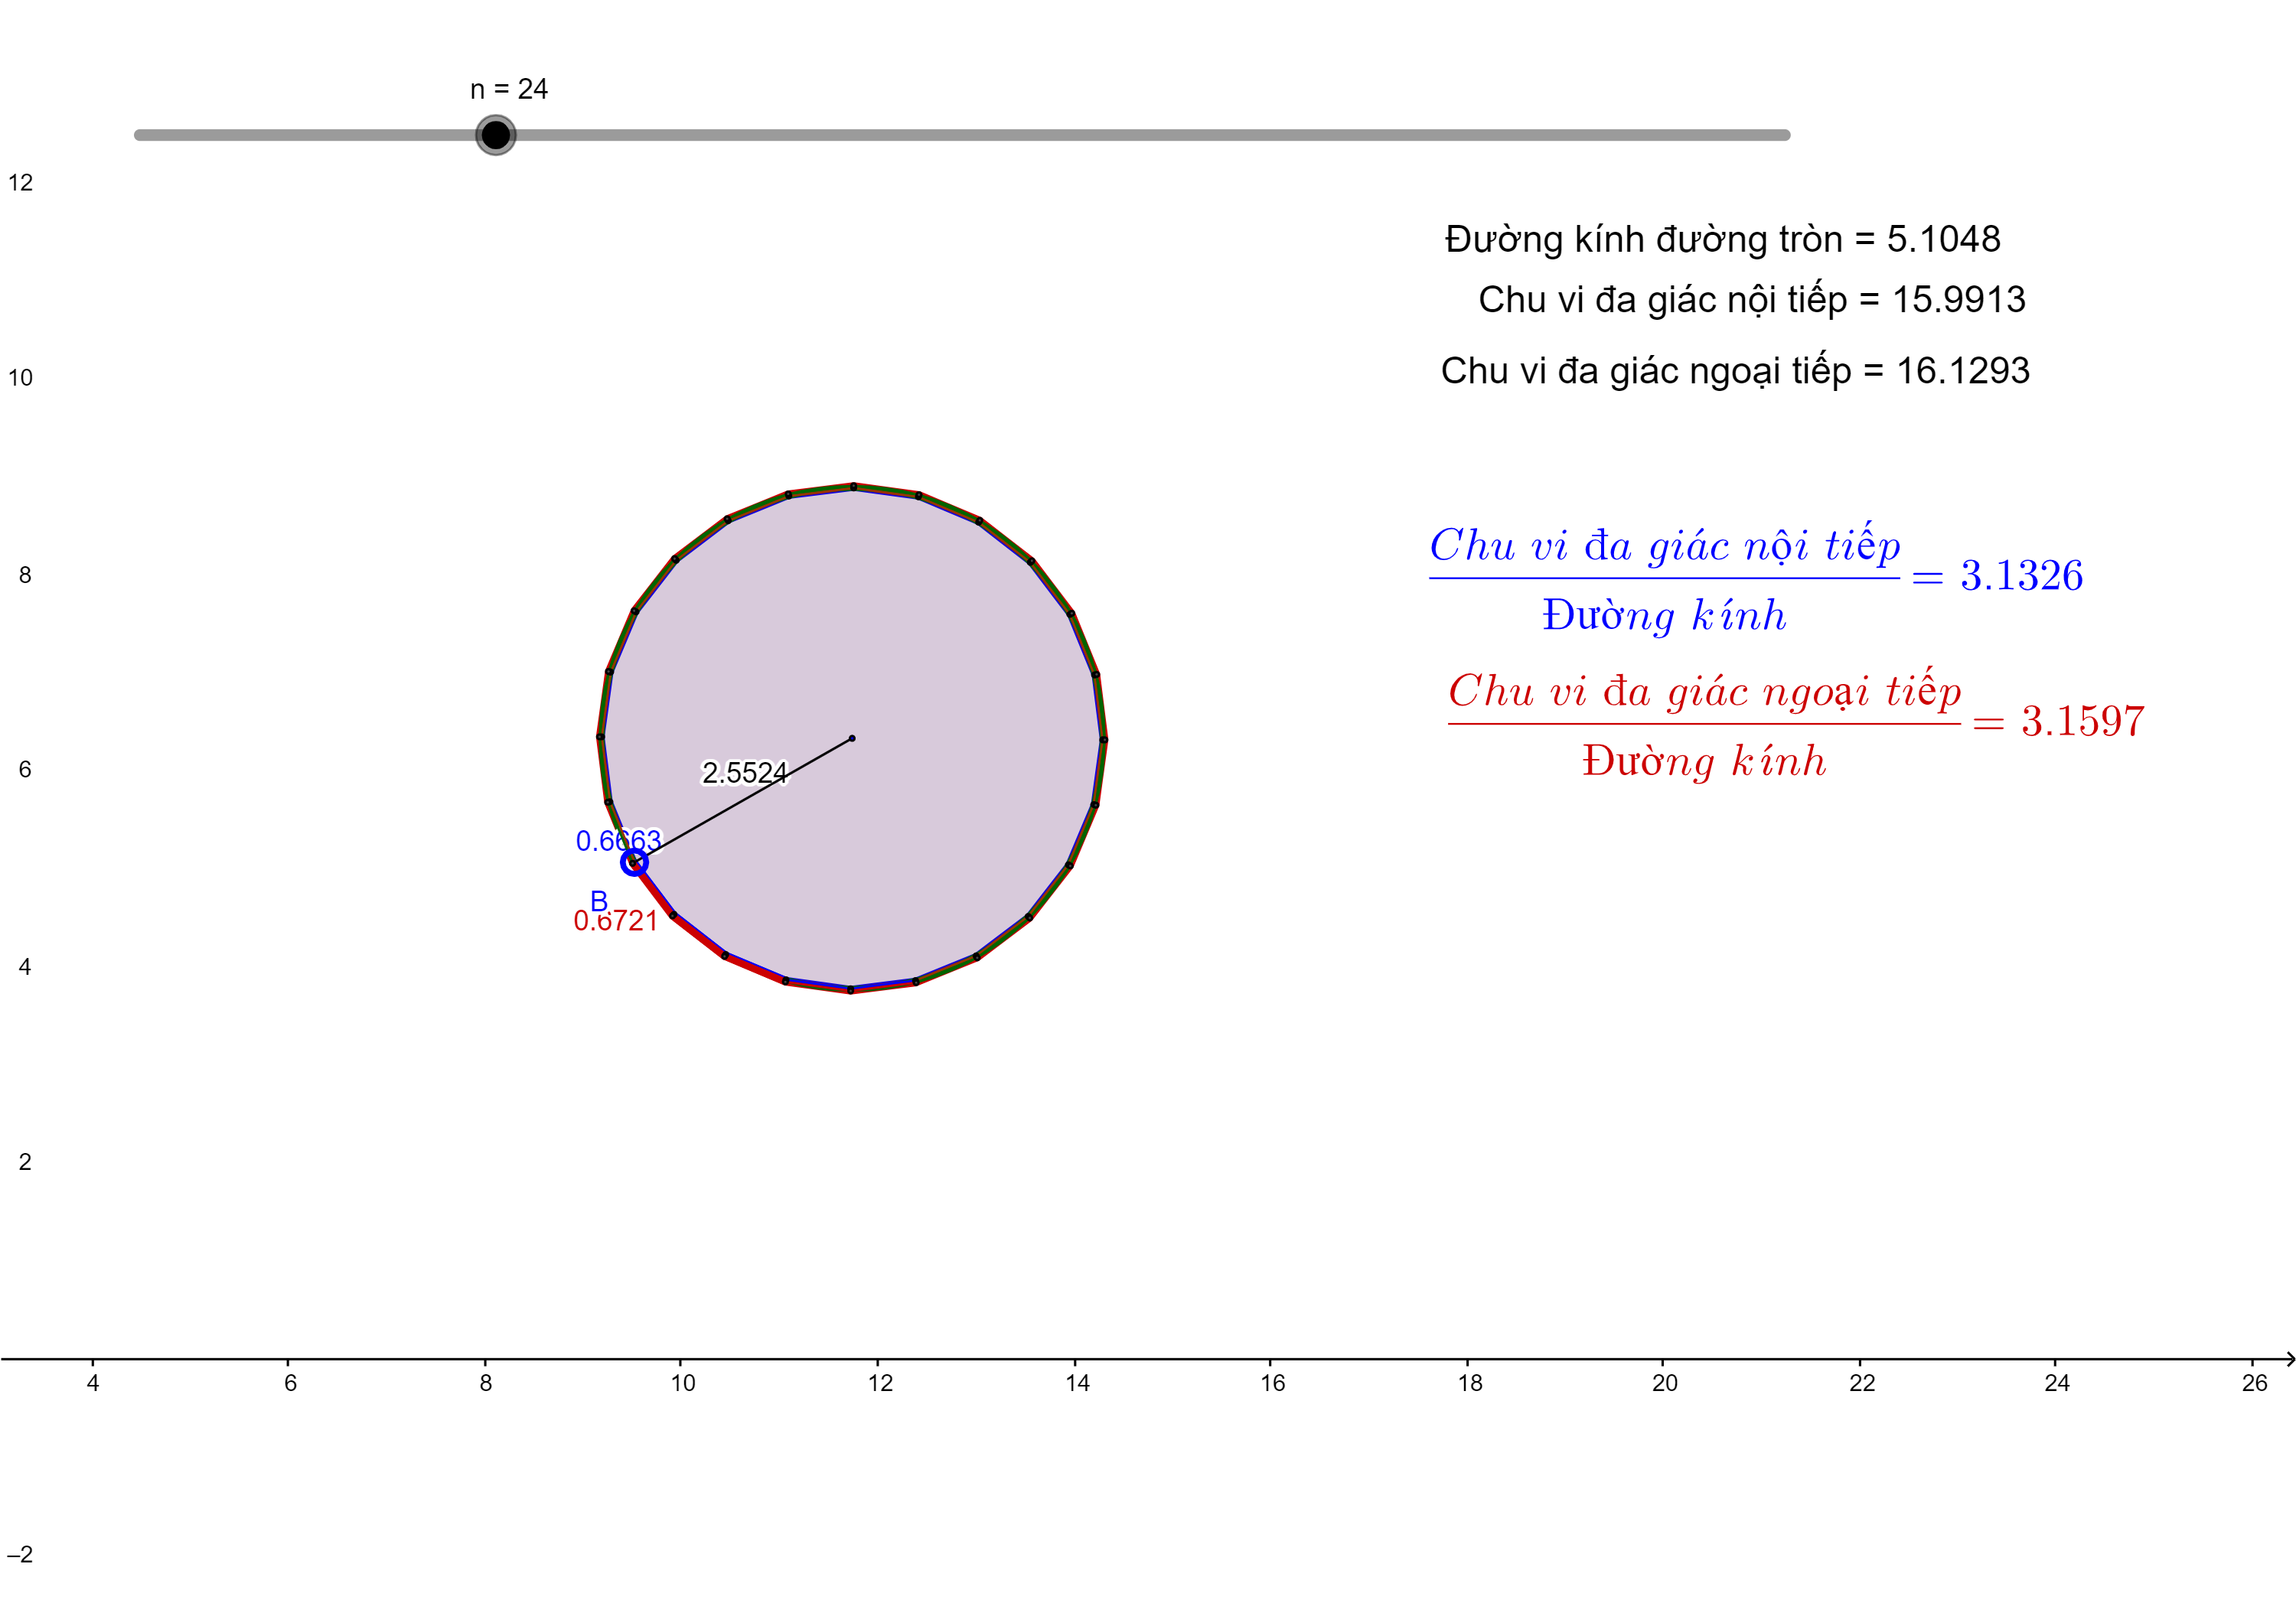
\includegraphics[width= 1\linewidth]{14}
		\caption{\small\textit{\color{lichsutoanhoc}$n = 24$.}}
			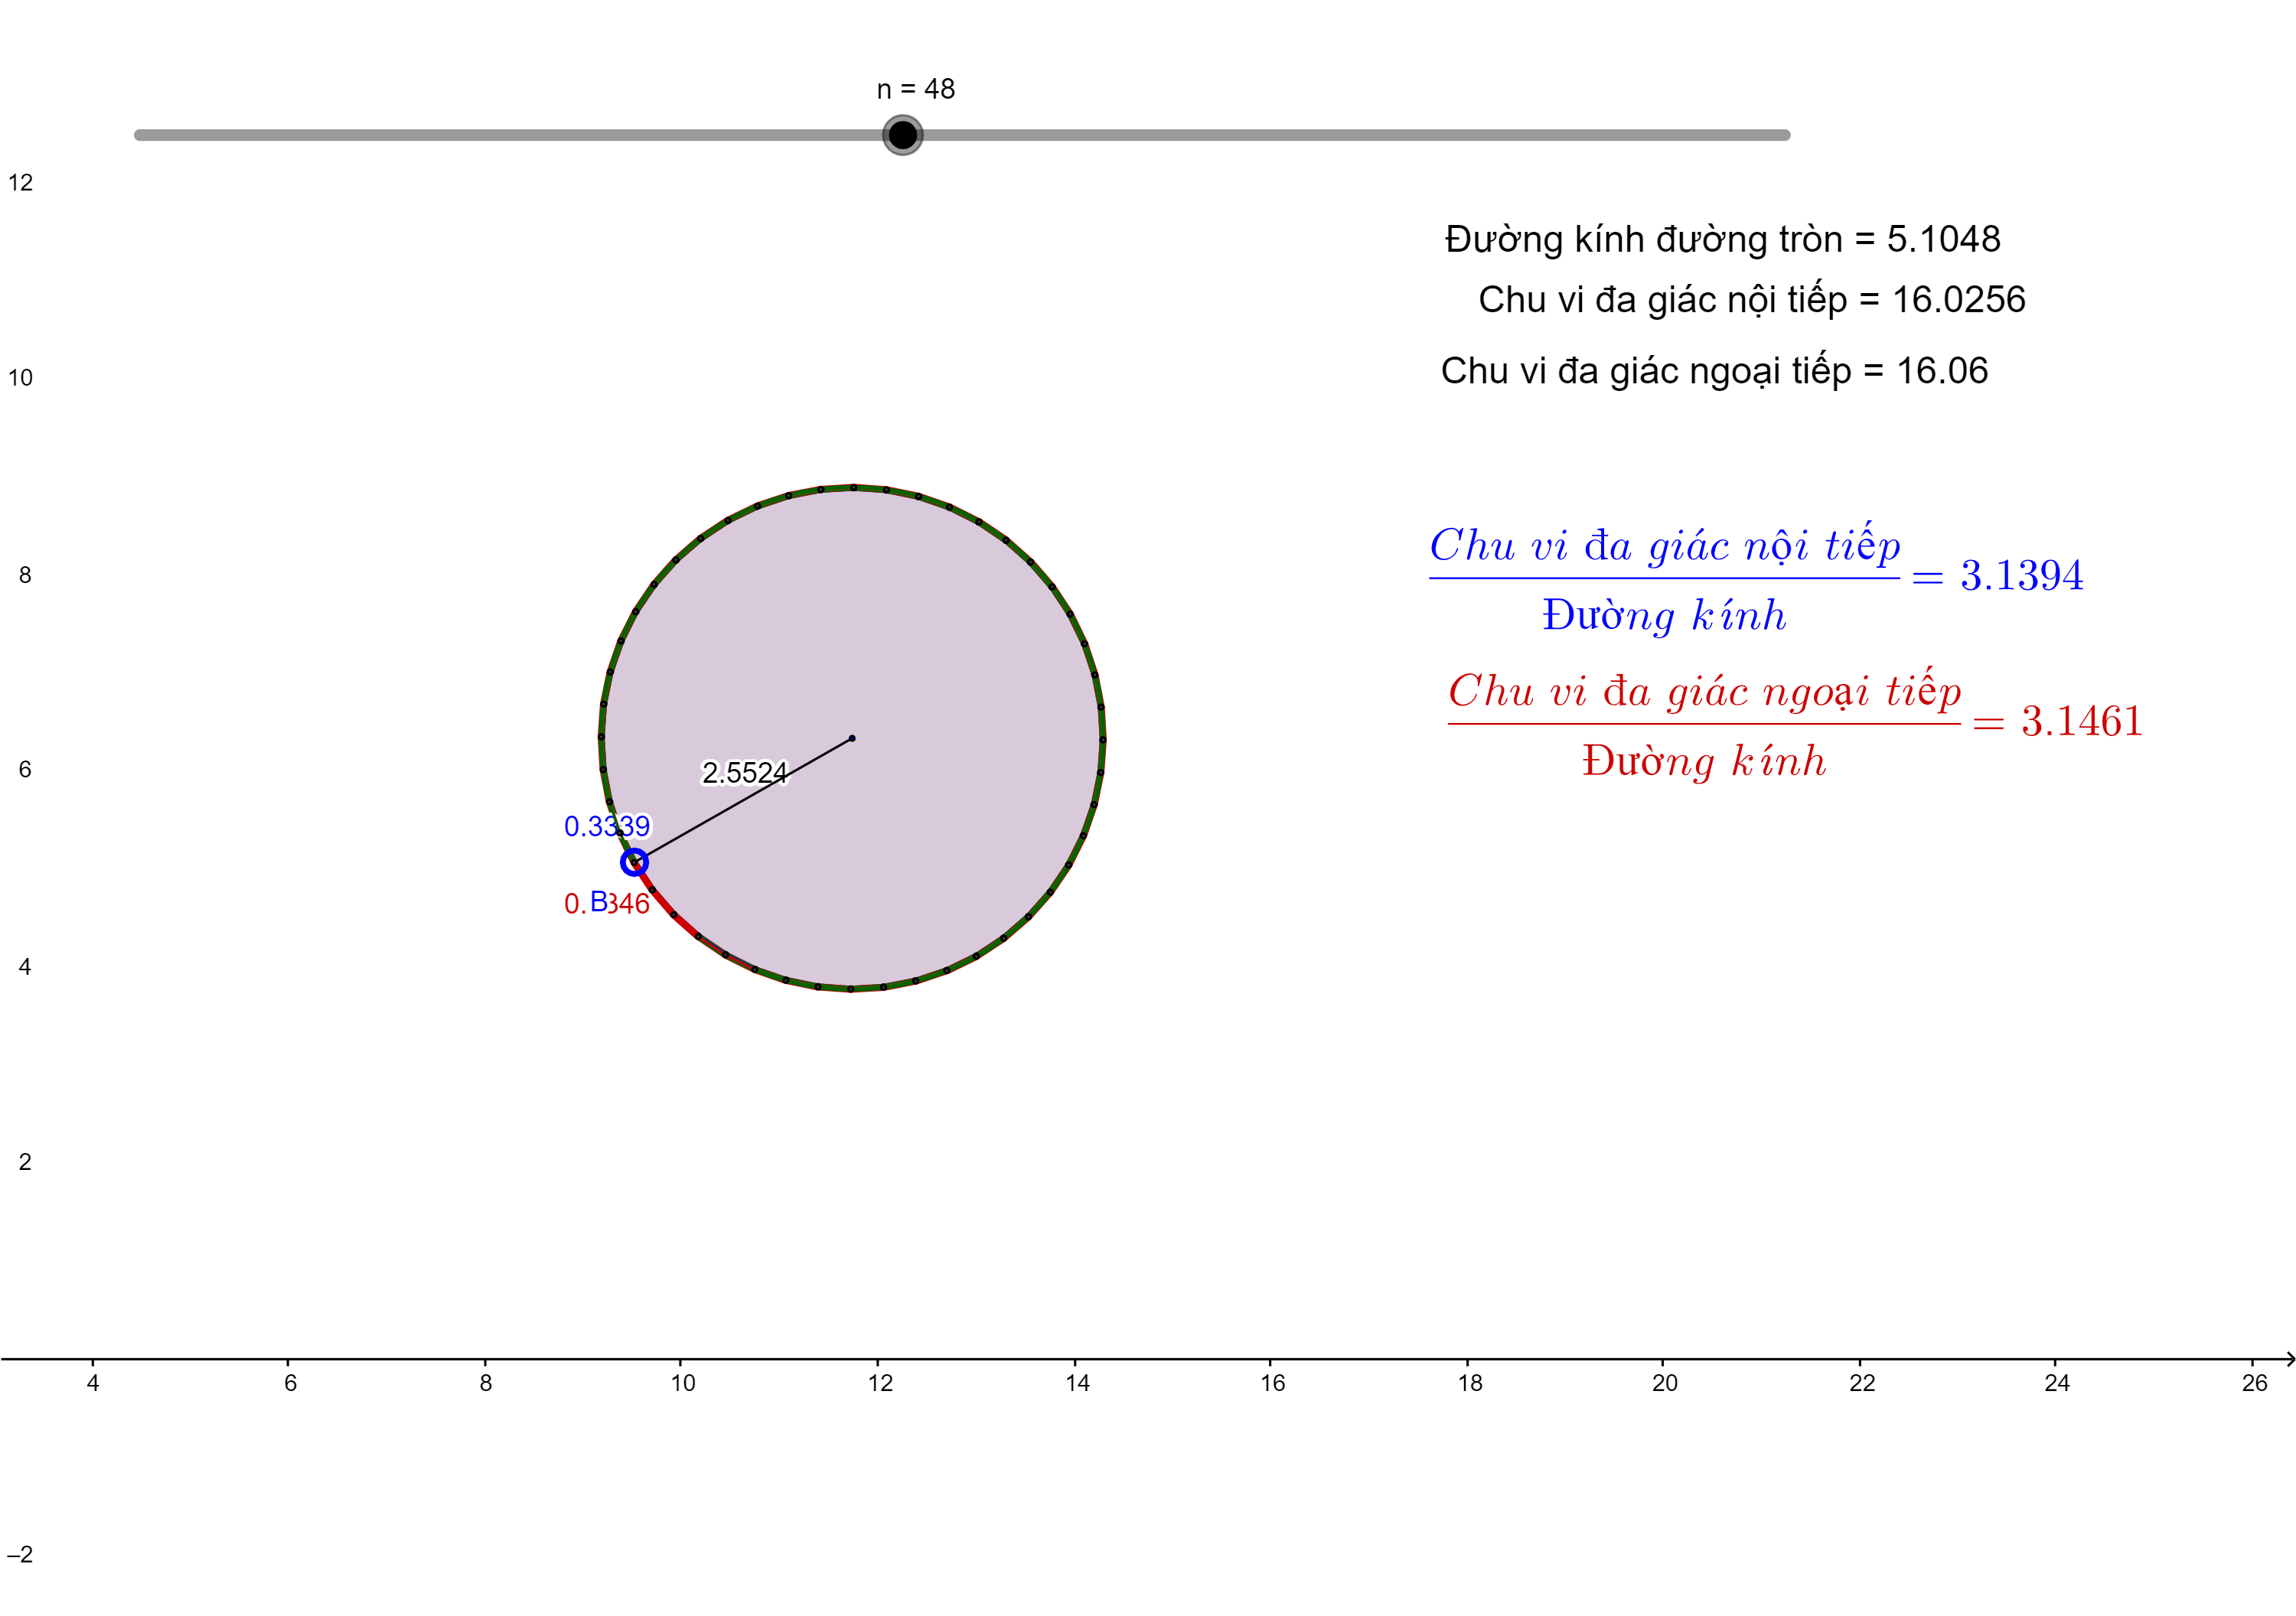
\includegraphics[width= 1\linewidth]{15}
		\caption{\small\textit{\color{lichsutoanhoc}$n = 48$.}}
		\vspace*{-10pt}
	\end{figure}
%	\begin{figure}[H]
%		\vspace*{-5pt}
%		\centering
%		\captionsetup{labelformat= empty, justification=centering}
%		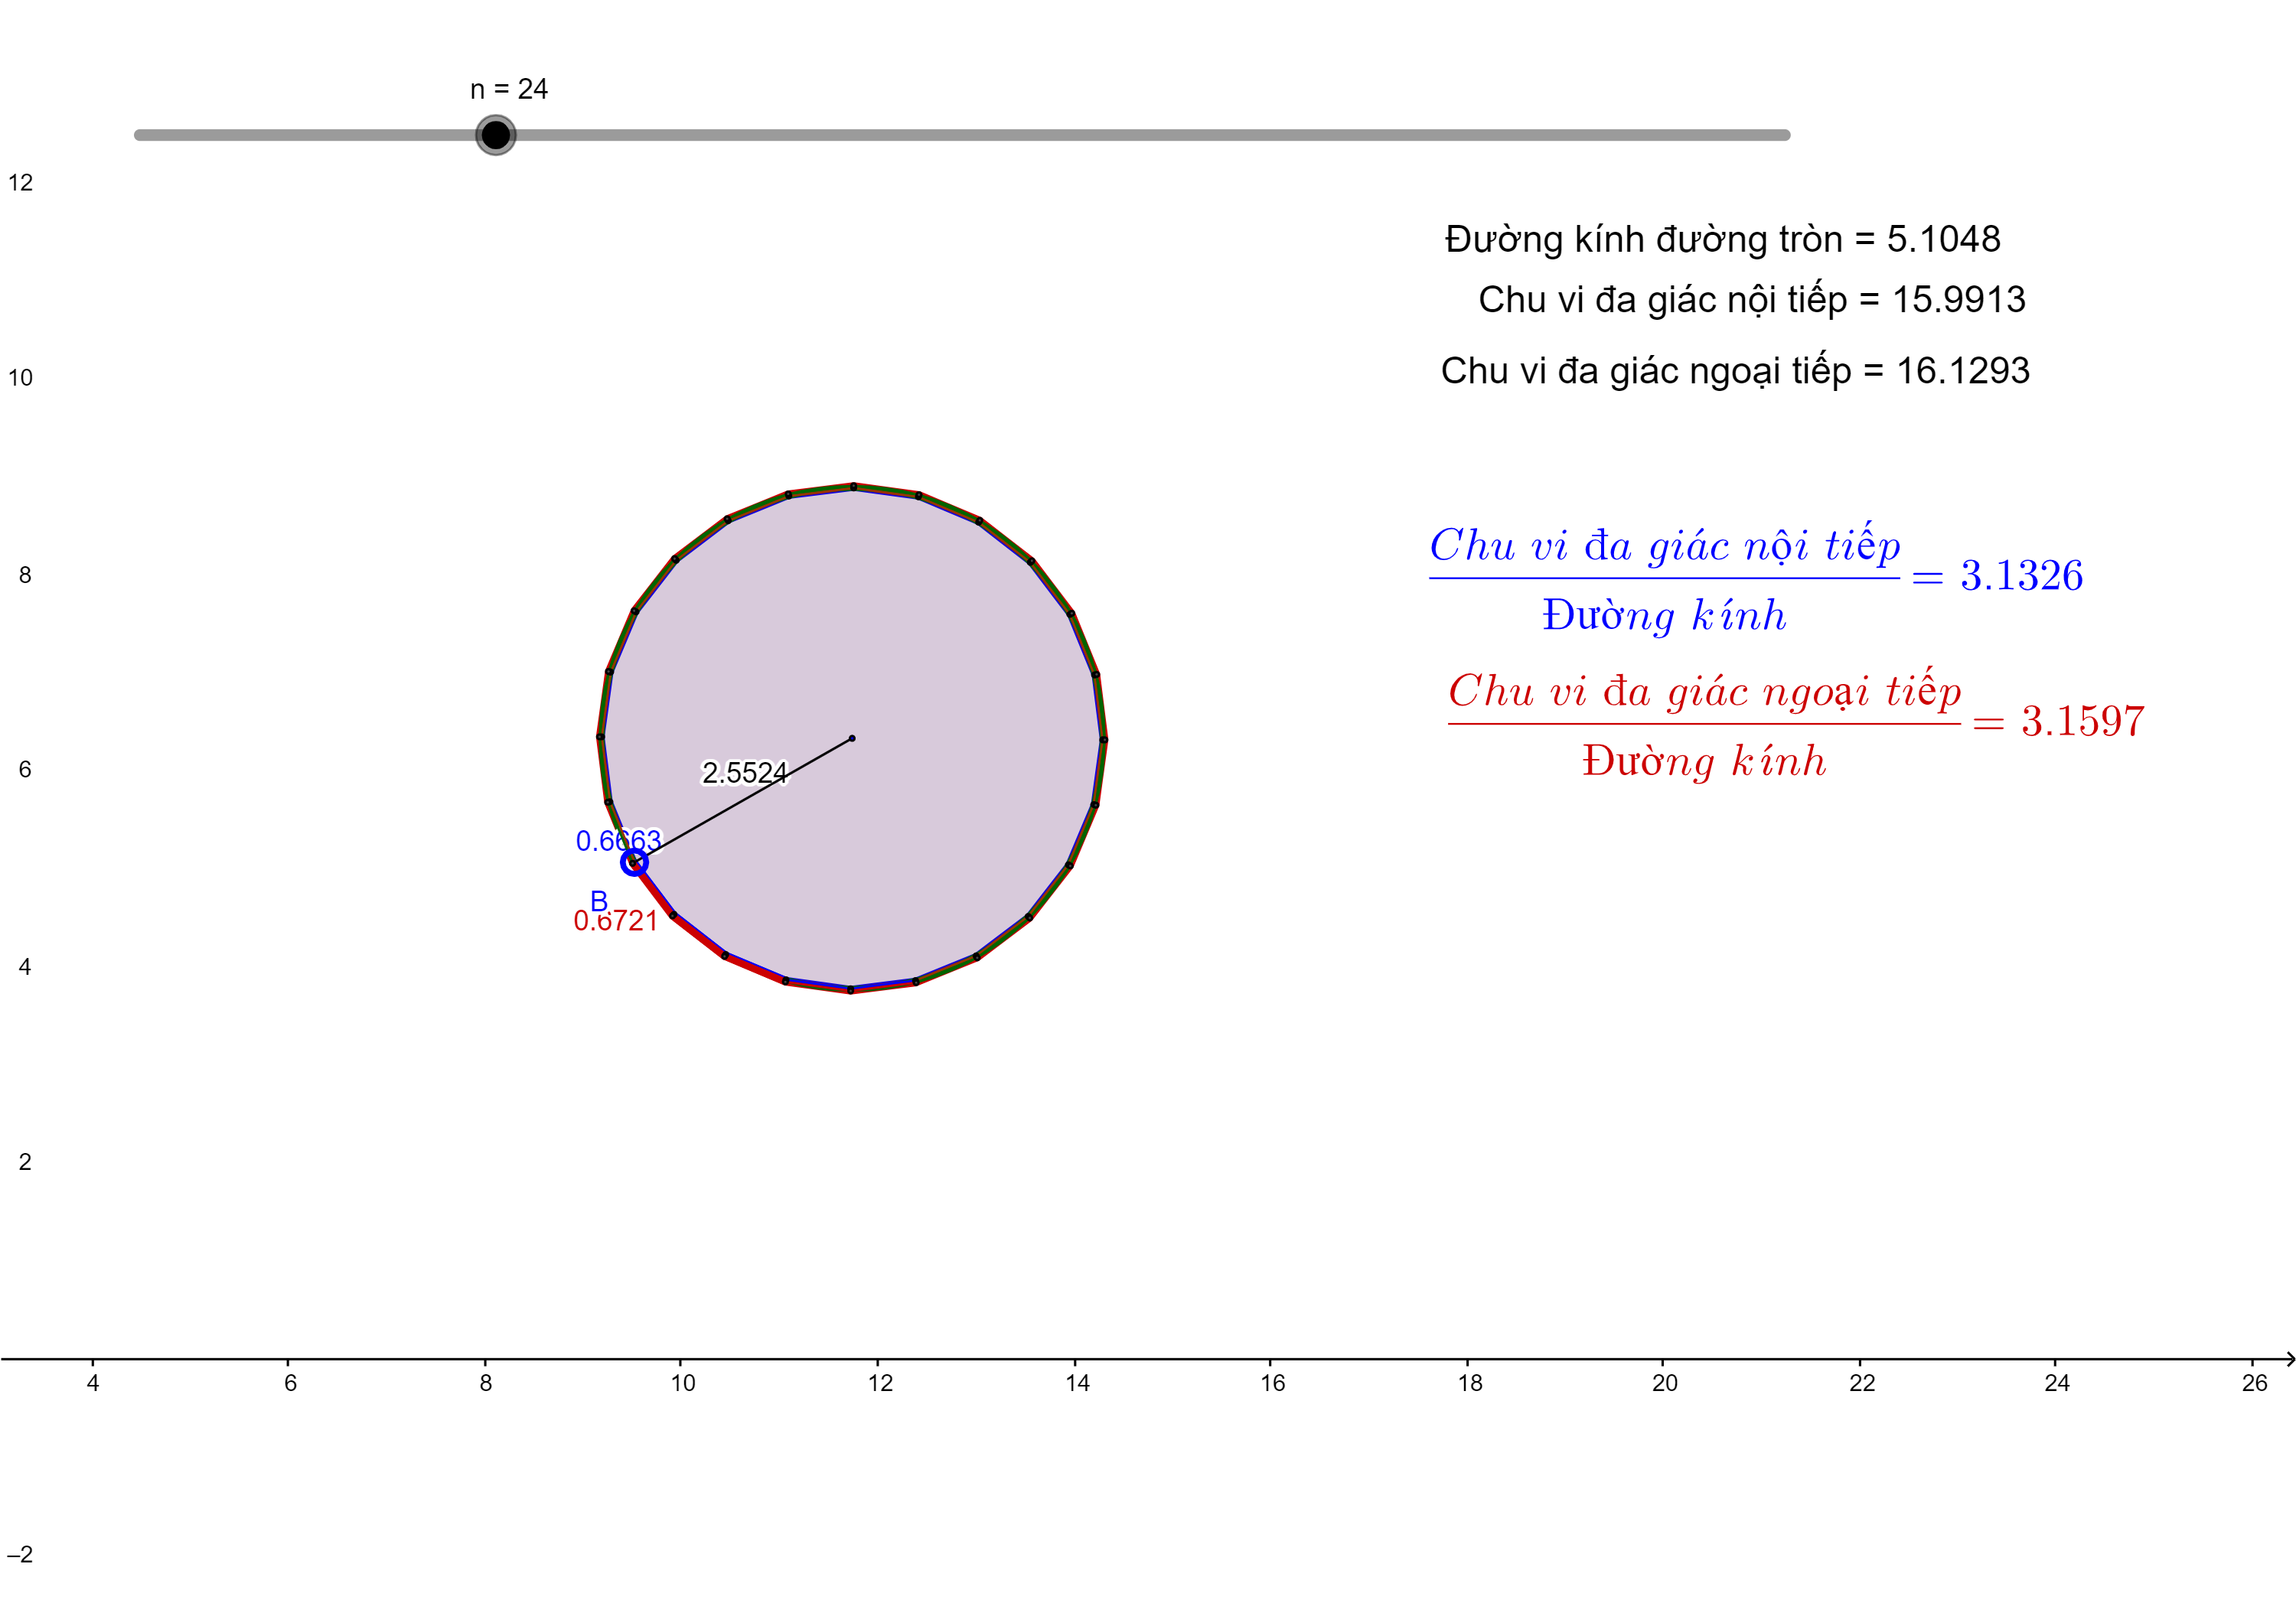
\includegraphics[width= 1\linewidth]{14}
%		\caption{\small\textit{\color{lichsutoanhoc}$n = 24$.}}
%		\vspace*{-10pt}
%	\end{figure}
%	\begin{figure}[H]
%		\vspace*{-5pt}
%		\centering
%		\captionsetup{labelformat= empty, justification=centering}
%		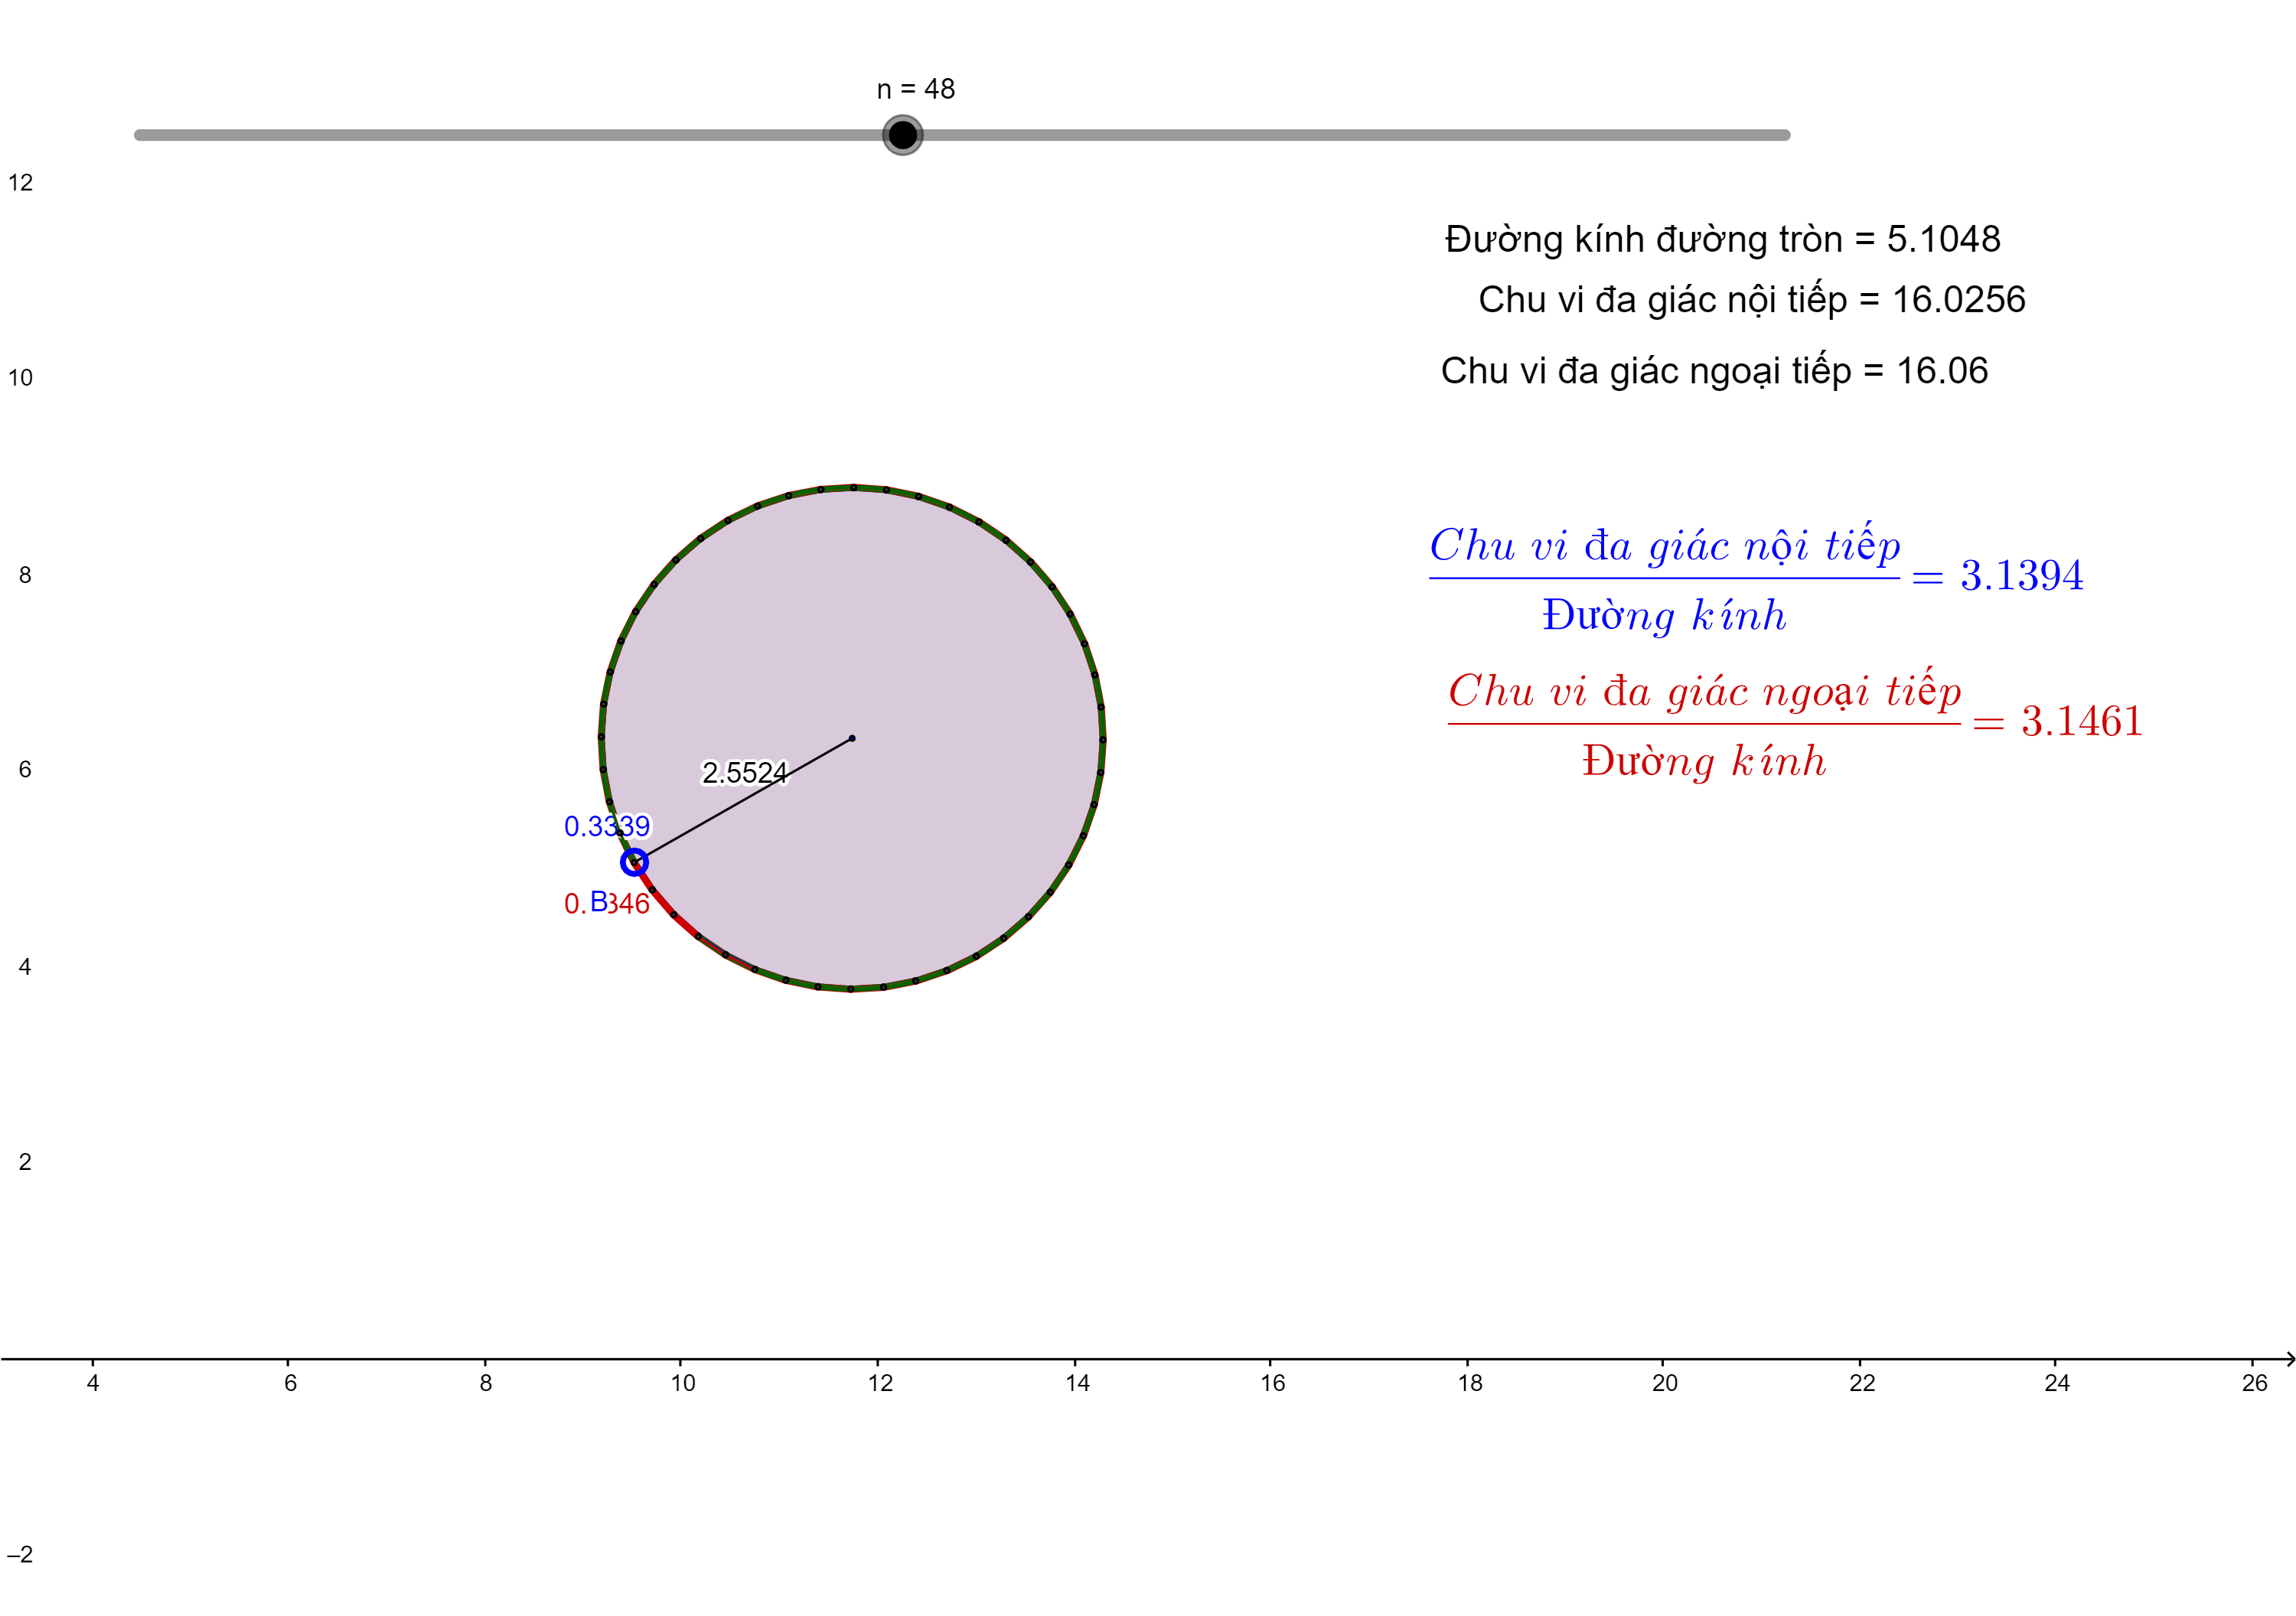
\includegraphics[width= 1\linewidth]{15}
%		\caption{\small\textit{\color{lichsutoanhoc}$n = 48$.}}
%		\vspace*{-10pt}
%	\end{figure}
	\begin{figure}[H]
		\vspace*{-5pt}
		\centering
		\captionsetup{labelformat= empty, justification=centering}
		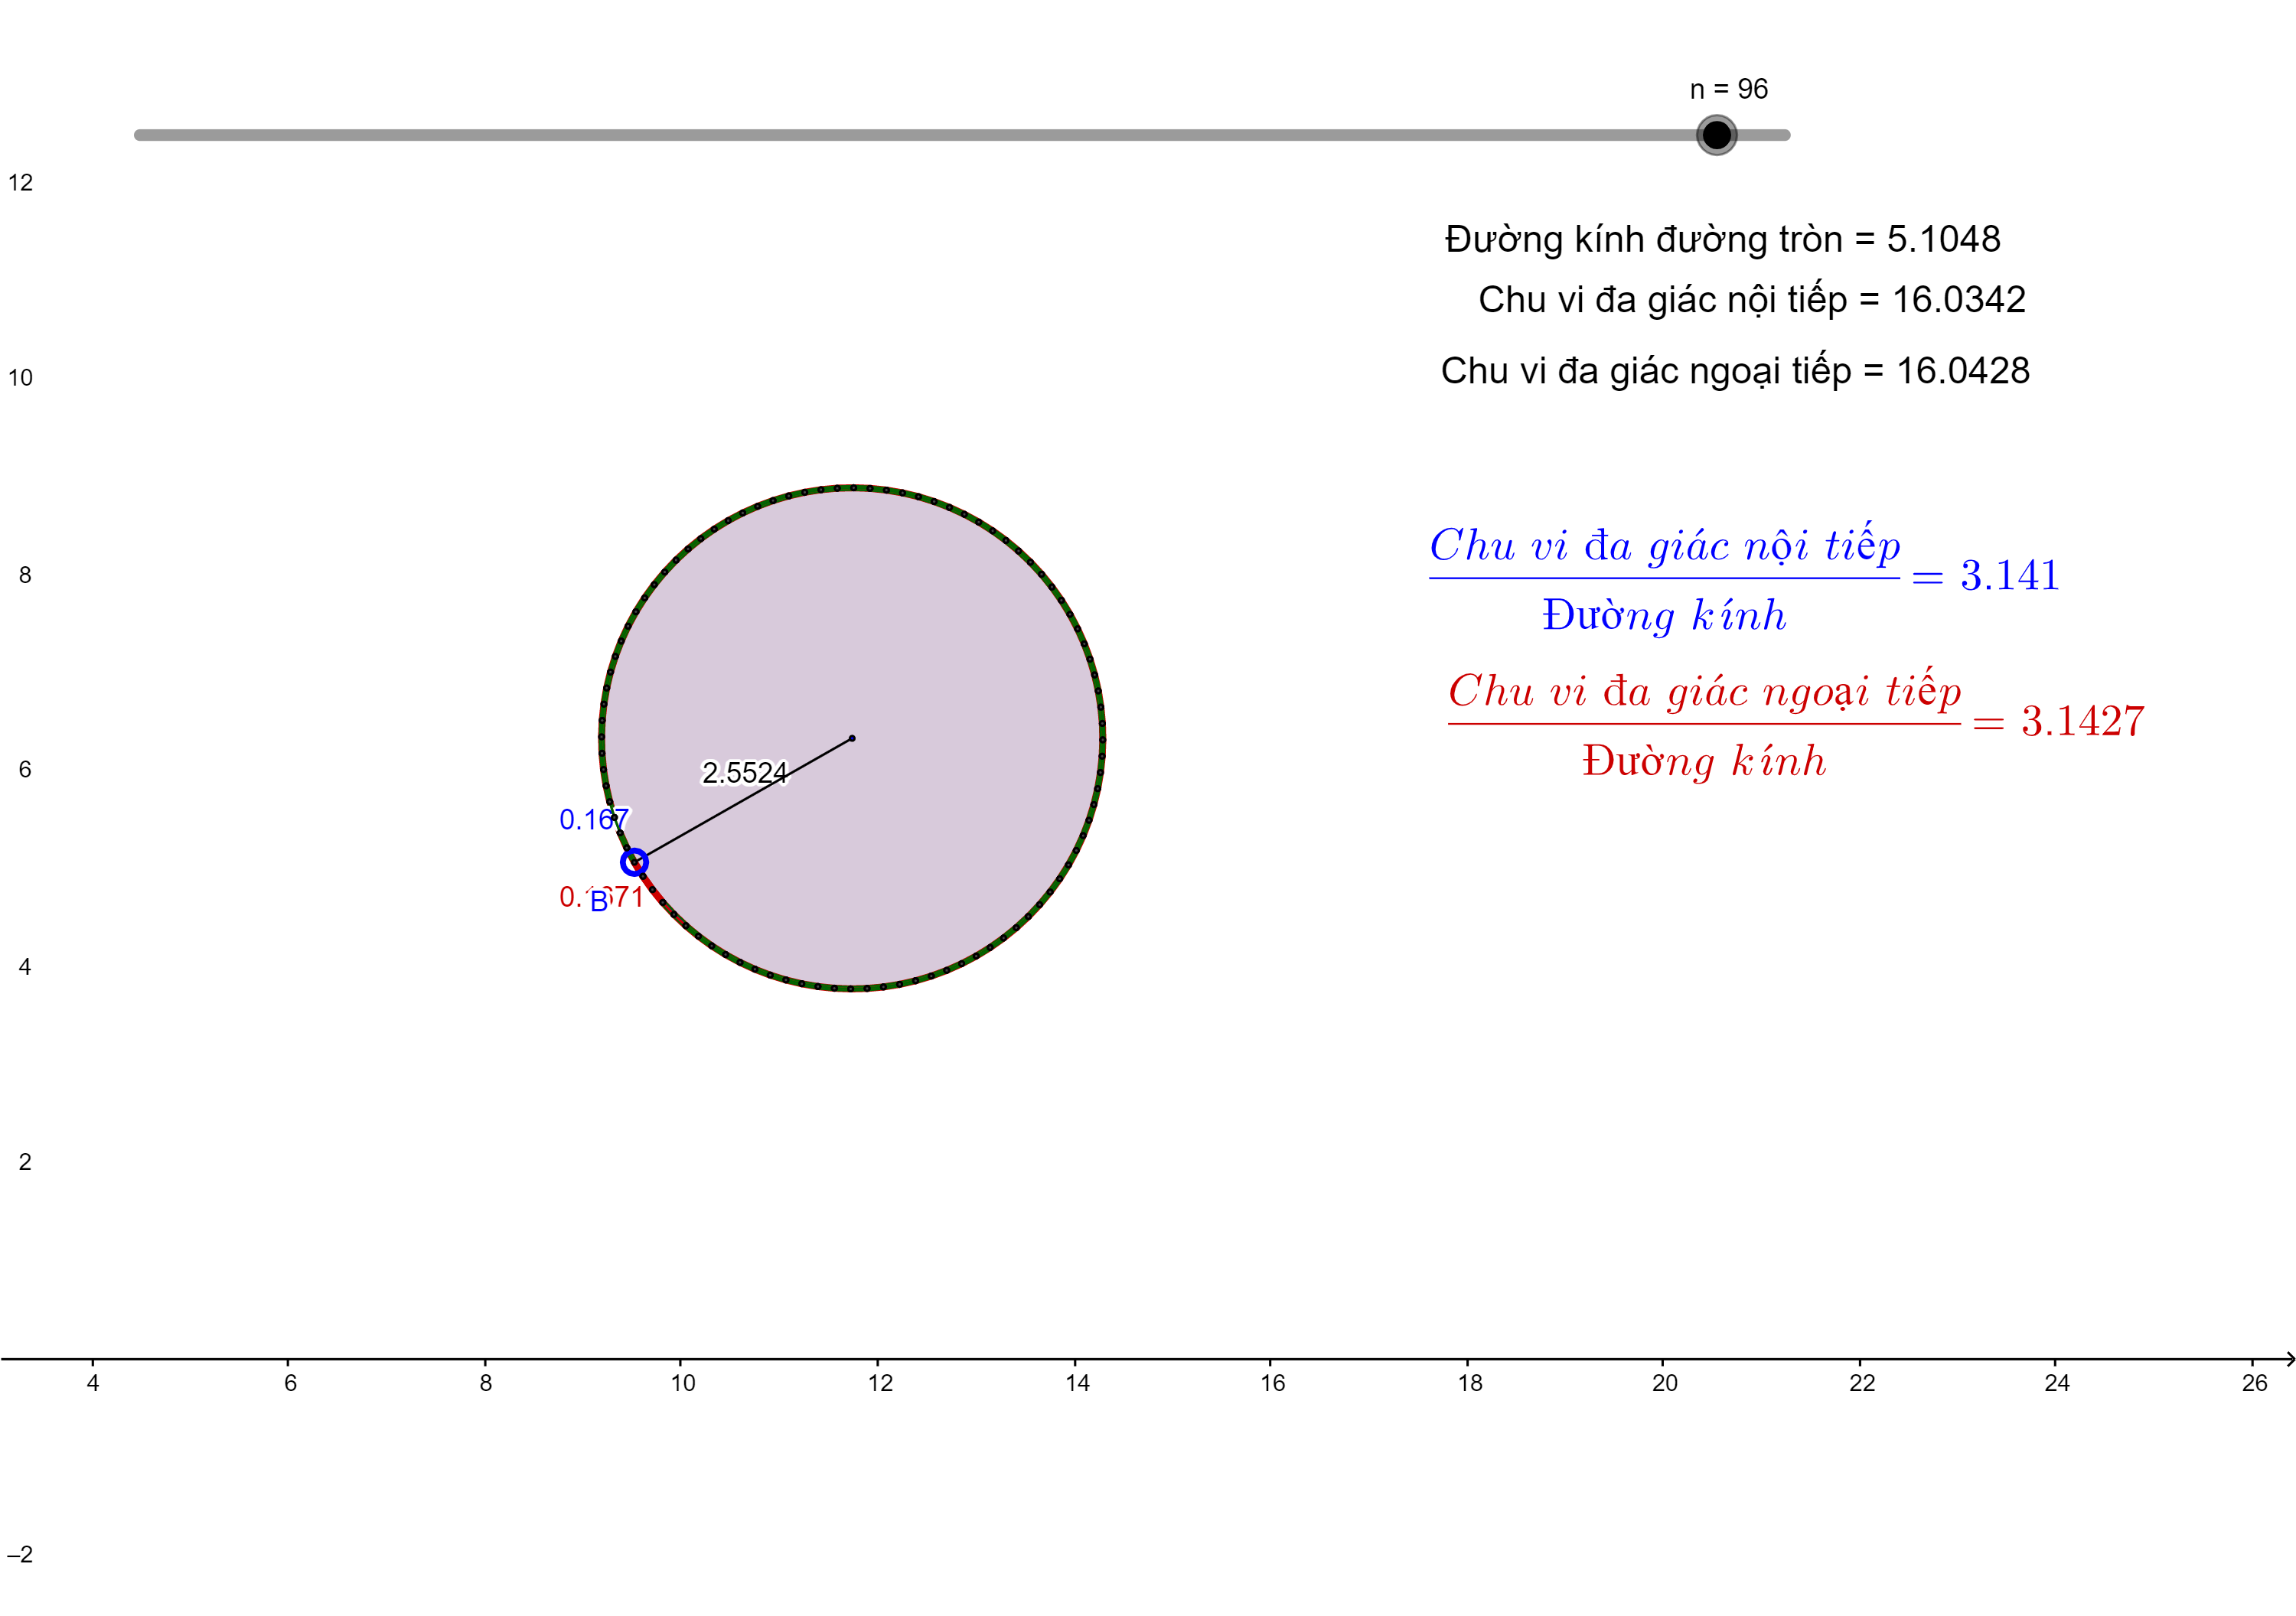
\includegraphics[width= 1\linewidth]{16}
		\caption{\small\textit{\color{lichsutoanhoc}$n = 96$.}}
		\vspace*{-10pt}
	\end{figure}	
	\textit{GeoGebra} đã cài đặt số Pi gần đúng đến $13$ chữ số $3.141592653589$.
	\vskip 0.1cm  
	Máy tính điện tử khoa học (Casio fx--$580$) đã cài đặt số Pi gần đúng đến $10$ chữ số
	\begin{align*}
		\pi \approx 3.141592653
	\end{align*}
	\textbf{\color{lichsutoanhoc}Thay lời kết}
	\vskip 0.1cm
	Xung quanh số $\pi$  còn khá nhiều điều đáng được quan tâm. Thí dụ:
	\vskip 0.1cm
	$1)$ Tính chất vô tỷ và siêu việt (không là nghiệm của phương trình đa thức) của số $\pi$.
	\vskip 0.1cm  
	$2)$ Biểu diễn số  $\pi$ qua phân số liên tục.
	\vskip 0.1cm
	$3)$ Các công thức mới, lập trình và tính gần đúng số $\pi$  trên các máy tính hiện đại. 
	\vskip 0.1cm
	$4)$ Phương pháp Monte--Carlo tính gần đúng $\pi$.
	\vskip 0.1cm   
	$5)$ Số $\pi$ và những vấn đề toán học liên quan (Công thức Euler, Hàm zeta, Fractal, \ldots).
	\vskip 0.1cm
	$6)$ Số $\pi$ trong cuộc sống, \ldots 
	\vskip 0.1cm
	Bạn đọc có thể tham khảo thêm trong các tài liệu [$2$], [$3$]  và trên Internet. 
	\vskip 0.1cm
	\textbf{\color{lichsutoanhoc}Tài liệu tham khảo}
	\vskip 0.1cm
	[$1$] Tạ Duy Phượng, Đoàn Thị Lệ, Cung Thị Kim Thành, Mai Văn Thu, Nguyễn Hoàng Vũ, Tính số Pi: Xưa và Nay, Phần $1$: Tính số Pi: Xưa, Tạp chí Pi, Tập $7$, số $3$, $2023$.
	\vskip 0.1cm
	[$2$] Petr Beckmann, \textit{A History of} $\pi$ (Pi), St. Martin's Press, New York, in lần thứ ba, $1974$.
	\vskip 0.1cm 
	[$3$] Lennart Berggren, Jonathan Borwein, Peter Borwein, Pi: \textit{A Source Book} (Second Edition), Springer, $2000$.
	\vskip 0.1cm 
	[$4$] Một số tư liệu trên Internet.
\end{multicols}